%***************************************************************************************************
% main.tex - szkielet dokumentu. Dane dokumentu edytuj w config/metadata.tex,
% treść w katalogu chapters/, a wygląd w preamble/ i config/theme-pwr.tex.
% Kompilacja: pdfLaTeX + BibTeX (na Overleaf: kompilator pdfLaTeX, plik główny main.tex).
%***************************************************************************************************

% Dla druku jednostronnego zamień "twoside" na "oneside".
\documentclass[11pt, a4paper, twoside, openany]{book}

% ============================== KONFIGURACJA I PREAMBUŁA ==============================
%***************************************************************************************************
% config/metadata.tex - JEDYNE miejsce, które edytujesz przy tworzeniu nowego dokumentu.
% Tytuł, przedmiot, autorzy, data oraz przełączniki opcjonalnych części dokumentu.
% Nie używaj tu \today - data i skrót na stronie tytułowej są wpisywane ręcznie.
%***************************************************************************************************

% ---------------------------------------------------------------------------------------------
% Dane dokumentu (widoczne na stronie tytułowej)
% ---------------------------------------------------------------------------------------------
\newcommand{\DocType}{Dokumentacja Projektowa}                       % np. Raport, Sprawozdanie, Projekt
\newcommand{\DocTitle}{Firewall w PowerShell - zarządzanie regułami zapory}             % tytuł (może być długi, zawija się)

\newcommand{\Course}{Cyberbezpieczeństwo}        % kierunek studiów
\newcommand{\Subject}{Ochrona Systemów Operacyjnych}             % przedmiot - pojawia się też w stopce każdej strony
\newcommand{\GroupInfo}{Grupa nr 4 / czwartek, godz. 17:05 - 19:40}

\newcommand{\AuthorsLabel}{Autorzy}                 % etykieta nad listą autorów (np. Autor)
\newcommand{\Authors}{%                             % linie rozdzielaj przez \\ (bez \\ na końcu)
    Aleh Shehda, nr albumu 272277\\
    Aliaksei Lapachuk, nr albumu 276711\\
    Adam Rola, nr albumu 272194\\
    Ruslan Hedz, nr albumu 272212
}

\newcommand{\SupervisorLabel}{Prowadzący}           % etykieta nad danymi prowadzącego
\newcommand{\Supervisor}{%
    mgr inż. Adrian Wojciech Florek
}

% Miejscowość i data - wpisywane ręcznie (świadomie bez \today).
\newcommand{\PlaceDate}{Wrocław, 2026}

% Linia ze skrótem na stronie tytułowej. Dowolny napis; pozostaw pusty (\newcommand{\DocumentHash}{}),
% aby ją ukryć. Domyślnie: skrót pustego ciągu danych (czysto dekoracyjny).
\newcommand{\DocumentHash}{4d765532542ad27ee8332d18c750238d7d4ec295ca117fb7aeca216a0339bdf0}

% Autor w metadanych pliku PDF (bez znaków \\ i adresów e-mail)
\newcommand{\PdfAuthor}{Aleh Shehda, Aliaksei Lapachuk, Adam Rola, Ruslan Hedz}

% ---------------------------------------------------------------------------------------------
% Przełączniki opcjonalnych części dokumentu: \...true = pokaż, \...false = ukryj
% ---------------------------------------------------------------------------------------------
\newif\ifshowabstract         \showabstractfalse          % Streszczenie przed spisem treści
\newif\ifshowabbreviations    \showabbreviationstrue      % Spis skrótów po spisie treści
\newif\ifshowbibliography     \showbibliographytrue       % Bibliografia (BibTeX, bib/references.bib)
\newif\ifshowlistoffigures    \showlistoffigurestrue      % Spis rysunków
\newif\ifshowlistoftables     \showlistoftablestrue       % Spis tabel
\newif\ifshowlistoflistings   \showlistoflistingstrue     % Spis listingów
\newif\ifshowlistofalgorithms \showlistofalgorithmsfalse  % Spis algorytmów
\newif\ifshowappendices       \showappendicesfalse        % Załączniki

% Wersja do druku: wyłącza kolorowe odnośniki w PDF (\printversiontrue)
\newif\ifprintversion         \printversionfalse

% Domyślne umiejscowienie rysunków wstawianych makrem \Figure
% (H = dokładnie w miejscu wywołania; htbp = pozwól LaTeX-owi przesuwać)
\newcommand{\DefaultFigurePlacement}{H}
          % dane dokumentu i przełączniki
%***************************************************************************************************
% preamble/packages.tex - lista pakietów w ustalonej kolejności.
% Kolejność ładowania jest istotna - nie zmieniaj jej bez potrzeby.
% Pakiet hyperref jest ładowany osobno, na samym końcu (preamble/links.tex).
%***************************************************************************************************

% ---------------------------------------------------------------------------------------------
% Język, kodowanie, czcionki, typografia (dokument wyłącznie w języku polskim)
% ---------------------------------------------------------------------------------------------
\usepackage[T1]{fontenc}
\usepackage[utf8]{inputenc}    % wymagane przez klucz inputencoding pakietu listings
\usepackage{lmodern}
\usepackage[polish]{babel}
\let\lll\undefined             % babel (polish) definiuje \lll, co koliduje z amssymb
\usepackage{csquotes}          % polskie cudzysłowy: \enquote{tekst}
\usepackage{indentfirst}       % wcięcie pierwszego akapitu po nagłówku (zwyczaj polski)
\usepackage{microtype}
\frenchspacing                 % polska typografia: jednakowe odstępy po kropce

% ---------------------------------------------------------------------------------------------
% Matematyka
% ---------------------------------------------------------------------------------------------
\usepackage{amsmath}
\usepackage{amssymb}
\usepackage{amsthm}
\usepackage{mathtools}

% ---------------------------------------------------------------------------------------------
% Kolory, grafika, obiekty pływające
% ---------------------------------------------------------------------------------------------
\usepackage[table, svgnames]{xcolor}
\usepackage{graphicx}
\usepackage{float}             % umożliwia [H] (dokładne umiejscowienie obiektu)
\usepackage{caption}
\usepackage{subcaption}        % podrysunki: środowisko subfigure

% ---------------------------------------------------------------------------------------------
% Tabele
% ---------------------------------------------------------------------------------------------
\usepackage{array}
\usepackage{tabularx}
\usepackage{booktabs}
\usepackage{longtable}
\usepackage{multirow}
\usepackage{makecell}
\usepackage{seqsplit}          % łamanie długich ciągów (np. skrótów SHA-256) w dowolnym miejscu

% ---------------------------------------------------------------------------------------------
% Listy, listingi, algorytmy, dołączanie PDF
% ---------------------------------------------------------------------------------------------
\usepackage{enumitem}
\usepackage{listings}
\usepackage[ruled, vlined, linesnumbered, shortend, algochapter]{algorithm2e}
\usepackage{pdfpages}          % \includepdf - wstawianie stron z plików PDF (np. do załączników)
\usepackage{multicol}
\usepackage{pifont}            % znaczniki \ding (\cmark, \xmark w makrach)

% ---------------------------------------------------------------------------------------------
% Układ strony, nagłówki i stopki, tytuły rozdziałów
% ---------------------------------------------------------------------------------------------
% Marginesy 25 mm; bindingoffset zostawia dodatkowe 5 mm na zszycie (przy druku dwustronnym).
\usepackage[a4paper, top=25mm, bottom=25mm, left=25mm, right=25mm,
            bindingoffset=5mm, headheight=30pt, headsep=12pt]{geometry}
\usepackage{fancyhdr}
\usepackage{titlesec}
        % pakiety (kolejność istotna)
%***************************************************************************************************
% config/theme-pwr.tex - motyw Politechniki Wrocławskiej: kolory, nazwy jednostek, logo.
% Plik ładowany po pakiecie xcolor. Zmiana uczelni = zmiana tego pliku i pliku logo.
%***************************************************************************************************

% Kolory
\definecolor{PWrRed}{RGB}{140, 0, 20}      % oficjalny bordowy PWr
\definecolor{lgray}{HTML}{9F9F9F}
\definecolor{dgray}{HTML}{5F5F5F}
\colorlet{Accent}{PWrRed}                  % kolor akcentu używany w całym szablonie

% Nazwy jednostek (nagłówki stron, strona tytułowa)
\newcommand{\University}{Politechnika Wrocławska}
\newcommand{\Faculty}{Wydział Informatyki i Telekomunikacji}

% Plik z logo (względem katalogu głównego projektu)
\newcommand{\LogoFile}{logos/logoPWr.png}
         % kolory, nazwy uczelni i wydziału, logo
%***************************************************************************************************
% preamble/polish.tex - WSZYSTKIE polskie napisy dokumentu w jednym miejscu.
% Ładowany po pakietach (listings, algorithm2e), których nazwy nadpisuje.
%***************************************************************************************************

% Nazwy używane w nagłówkach spisów i podpisach
\newcommand{\abbrevname}{Spis skrótów}

\addto\captionspolish{%
  \renewcommand{\contentsname}{Spis treści}%
  \renewcommand{\listfigurename}{Spis rysunków}%
  \renewcommand{\listtablename}{Spis tabel}%
  \renewcommand{\lstlistlistingname}{Spis listingów}%
  \renewcommand{\chaptername}{Rozdział}%
  \renewcommand{\appendixname}{Załącznik}%
  \renewcommand{\bibname}{Bibliografia}%
  \renewcommand{\refname}{Bibliografia}%
  \renewcommand{\figurename}{Rysunek}%
  \renewcommand{\tablename}{Tabela}%
  \renewcommand{\lstlistingname}{Listing}%
  \renewcommand{\proofname}{Dowód}%
}

% Algorytmy (algorithm2e): nazwa środowiska, nazwa w odwołaniach i tytuł spisu
\SetAlgorithmName{Algorytm}{algorytm}{Spis algorytmów}
\SetAlFnt{\footnotesize}
\SetAlCapFnt{\small}
\SetAlCapNameFnt{\small\bfseries}

% Słowa kluczowe w pseudokodzie (algorithm2e)
\SetKwInOut{Input}{Dane wejściowe}
\SetKwInOut{Output}{Wynik}
\SetKwIF{If}{ElseIf}{Else}{jeżeli}{to}{w p.p. jeżeli}{w p.p.}{}
\SetKwFor{For}{dla}{wykonaj}{}
\SetKwFor{While}{dopóki}{wykonuj}{}
\SetKw{Return}{zwróć}
          % polskie napisy dokumentu
%***************************************************************************************************
% preamble/macros.tex - makra pomocnicze, środowiska matematyczne, pytania i odpowiedzi, listy.
%***************************************************************************************************

% ---------------------------------------------------------------------------------------------
% Makra semantyczne
% ---------------------------------------------------------------------------------------------
\newcommand{\code}[1]{\texttt{\detokenize{#1}}}
\newcommand{\file}[1]{\texttt{\detokenize{#1}}}
\newcommand{\cmd}[1]{\texttt{\detokenize{#1}}}
\newcommand{\latexcmd}[1]{\texttt{\textbackslash #1}}
\newcommand{\hash}[1]{{\ttfamily\footnotesize\seqsplit{#1}}}

\newcommand{\lead}[1]{\par\medskip\noindent\textbf{#1}\par\nopagebreak\smallskip}

\newcommand{\UnnumberedChapter}[1]{%
  \clearpage\phantomsection
  \addcontentsline{toc}{chapter}{#1}%
  \chapter*{#1}%
}

\newcounter{qacount}
\newenvironment{qa}[1]{%
  \refstepcounter{qacount}%
  \par\medskip\noindent\textbf{Pytanie \theqacount:} \textit{#1}\par\nopagebreak\smallskip
  \noindent\textbf{Odpowiedź}\par\nopagebreak
}{\par\medskip}

\newenvironment{abbreviations}
  {\begin{description}[style=multiline, leftmargin=3.5cm, font=\bfseries, itemsep=2pt]}
  {\end{description}}

\newcommand{\textapprox}{\raisebox{0.5ex}{\texttildelow}}

\newcommand{\cmark}{\ding{51}}
\newcommand{\xmark}{\ding{55}}
\newcommand{\hcell}[1]{\textbf{#1}}

% ---------------------------------------------------------------------------------------------
% Skróty matematyczne
% ---------------------------------------------------------------------------------------------
\newcommand{\NN}{\mathbb{N}}
\newcommand{\ZZ}{\mathbb{Z}}
\newcommand{\QQ}{\mathbb{Q}}
\newcommand{\RR}{\mathbb{R}}
\newcommand{\CC}{\mathbb{C}}
\newcommand{\IMP}{\rightarrow}
\newcommand{\IFF}{\leftrightarrow}

% ---------------------------------------------------------------------------------------------
% Twierdzenia, definicje, przykłady, uwagi
% ---------------------------------------------------------------------------------------------
\theoremstyle{plain}
\newtheorem{theorem}{Twierdzenie}[chapter]
\newtheorem{lemma}[theorem]{Lemat}
\newtheorem{corollary}[theorem]{Wniosek}

\theoremstyle{definition}
\newtheorem{definition}[theorem]{Definicja}
\newtheorem{example}[theorem]{Przykład}

\theoremstyle{remark}
\newtheorem{remark}[theorem]{Uwaga}

\renewcommand{\qedsymbol}{$\blacklozenge$}

% ---------------------------------------------------------------------------------------------
% Listy
% ---------------------------------------------------------------------------------------------
\setlist{topsep=0.4em, itemsep=0.2em, parsep=0pt, partopsep=0pt}
\setlist[itemize,1]{label=\textbullet, leftmargin=*}
\setlist[itemize,2]{label=-, leftmargin=*}
\setlist[itemize,3]{label=$\diamond$, leftmargin=*}
\setlist[enumerate,1]{label=\arabic*., leftmargin=*}
\setlist[enumerate,2]{label=\alph*), leftmargin=*}

\setlength{\emergencystretch}{2em}
          % makra, twierdzenia, listy
%***************************************************************************************************
% preamble/floats-and-tables.tex - podpisy, rysunki, tabele.
%***************************************************************************************************

\graphicspath{{images/}{logos/}}

\captionsetup{font=small, labelfont=bf, labelsep=period, skip=5pt}
\captionsetup[figure]{position=bottom}
\captionsetup[table]{position=top}
\captionsetup[subfigure]{font=footnotesize, labelfont=bf, labelsep=period, skip=3pt}

\floatplacement{figure}{htbp}
\setlength{\intextsep}{8pt plus 2pt minus 2pt}
\setlength{\textfloatsep}{10pt plus 2pt minus 2pt}
\setlength{\floatsep}{8pt plus 2pt minus 2pt}

\renewcommand{\topfraction}{0.92}
\renewcommand{\bottomfraction}{0.85}
\setcounter{topnumber}{3}
\setcounter{bottomnumber}{3}
\setcounter{totalnumber}{4}
\renewcommand{\textfraction}{0.06}
\renewcommand{\floatpagefraction}{0.85}

\raggedbottom

\makeatletter
\setlength\@fptop{0\p@}
\makeatother

% ---------------------------------------------------------------------------------------------
% Rysunek: \Figure[szerokość]{plik}{podpis}{etykieta}
% ---------------------------------------------------------------------------------------------
\newcommand{\Figure}[4][1.0]{%
  \begin{figure}[H]
    \centering
    \IfFileExists{images/#2}{%
      \includegraphics[width=#1\linewidth, keepaspectratio]{images/#2}%
    }{%
      \PackageWarning{oss-fw-project}{Brak pliku obrazu images/#2}%
      \fbox{\parbox[c][5cm][c]{0.8\linewidth}{\centering\textit{Brak pliku obrazu}\\[1ex]\texttt{\detokenize{images/#2}}}}%
    }%
    \caption{#3}\label{#4}%
  \end{figure}%
}

% ---------------------------------------------------------------------------------------------
% Tabele
% ---------------------------------------------------------------------------------------------
\newcommand{\tablefont}{\footnotesize}
\renewcommand{\arraystretch}{1.08}
\setlength{\tabcolsep}{5pt}

\newcolumntype{L}[1]{>{\raggedright\arraybackslash}p{#1}}
\newcolumntype{C}[1]{>{\centering\arraybackslash}m{#1}}
\newcolumntype{R}[1]{>{\raggedleft\arraybackslash}p{#1}}
\newcolumntype{Y}{>{\raggedright\arraybackslash}X}
\newcolumntype{Z}{>{\centering\arraybackslash}X}

%***************************************************************************************************
% preamble/listings.tex - jeden wspólny styl listingów (kod i wyjście terminala).
% Użycie: \begin{lstlisting}[caption={Opis}, label={lst:etykieta}] ... \end{lstlisting}
%         \begin{lstlisting}[style=code, language=PowerShell, ...] ... \end{lstlisting}
%         \lstinputlisting[style=code, language=PowerShell, caption={...}, label={...}]{plik.ps1}
%***************************************************************************************************

% Polskie znaki w listingach (pdfLaTeX + UTF-8); mapowanie zdefiniowane tylko tutaj
\lstset{
  inputencoding=utf8,
  extendedchars=true,
  literate=
    {ą}{{\k{a}}}1 {ć}{{\'c}}1 {ę}{{\k{e}}}1 {ł}{{\l{}}}1 {ń}{{\'n}}1
    {ó}{{\'o}}1 {ś}{{\'s}}1 {ź}{{\'z}}1 {ż}{{\.z}}1
    {Ą}{{\k{A}}}1 {Ć}{{\'C}}1 {Ę}{{\k{E}}}1 {Ł}{{\L{}}}1 {Ń}{{\'N}}1
    {Ó}{{\'O}}1 {Ś}{{\'S}}1 {Ź}{{\'Z}}1 {Ż}{{\.Z}}1
}

% Definicja języka PowerShell dla pakietu listings
\lstdefinelanguage{PowerShell}{
  morekeywords=[1]{function,if,else,elseif,switch,while,for,foreach,in,do,until,break,continue,return,try,catch,finally,throw,param,begin,process,end,filter,class,enum},
  morekeywords=[2]{Get-NetFirewallRule,New-NetFirewallRule,Set-NetFirewallRule,Remove-NetFirewallRule,Enable-NetFirewallRule,Disable-NetFirewallRule,Get-NetFirewallProfile,Set-NetFirewallProfile,Get-NetFirewallAddressFilter,Get-NetFirewallPortFilter,Get-NetConnectionProfile,Write-Host,Read-Host,Clear-Host,Select-Object,Where-Object,ForEach-Object,Sort-Object,Format-Table,Out-Null,Out-File,Add-Content,Get-Content,Test-Path,Get-Date,Export-Csv,Import-Csv,ConvertTo-Json,ConvertFrom-Json},
  sensitive=false,
  morecomment=[l]{\#},
  morecomment=[s]{<\#}{\#>},
  morestring=[b]",
  morestring=[b]',
  alsoletter={-}
}

% Styl bazowy
\lstdefinestyle{base}{
  basicstyle=\ttfamily\footnotesize,
  columns=fullflexible,
  keepspaces=true,
  frame=single,
  rulecolor=\color{lgray},
  breaklines=true,
  postbreak=\mbox{\textcolor{dgray}{$\hookrightarrow$}\space},
  showstringspaces=false,
  captionpos=t,
  aboveskip=1em,
  belowskip=1em,
}

% Wyjście terminala / sesja konsoli (styl domyślny)
\lstdefinestyle{terminal}{
  style=base,
  backgroundcolor=\color{gray!6},
}

% Kod źródłowy (z numerami wierszy i kolorami)
\lstdefinestyle{code}{
  style=base,
  numbers=left,
  numberstyle=\tiny\color{dgray},
  numbersep=6pt,
  xleftmargin=1.6em,
  framexleftmargin=1.6em,
  keywordstyle=[1]\bfseries\color{Accent},
  keywordstyle=[2]\bfseries\color{NavyBlue},
  commentstyle=\itshape\color{dgray},
  stringstyle=\color{DarkGreen},
}

\lstset{style=terminal}

% Numeracja listingów w obrębie rozdziału (jak rysunki i tabele)
\AtBeginDocument{\counterwithin{lstlisting}{chapter}}

%***************************************************************************************************
% preamble/headings.tex - formatowanie tytułów rozdziałów i sekcji, głębokość numeracji i spisu treści.
%***************************************************************************************************

\setcounter{secnumdepth}{3}    % numerujemy do poziomu \subsubsection
\setcounter{tocdepth}{1}       % w spisie treści do poziomu \section (zwięzły spis na 1 stronie)

% Etykieta przed tytułem rozdziału (w załącznikach zmieniana przez \StartAppendices)
\newcommand{\ChapterLabel}{\thechapter.}

\titleformat{\chapter}[hang]
  {\normalfont\huge\bfseries\raggedright}{\ChapterLabel}{1ex}{}
\titlespacing*{\chapter}{0pt}{0pt}{16pt}

\titleformat{\section}[hang]
  {\normalfont\Large\bfseries\raggedright}{\thesection.}{1ex}{}
\titlespacing*{\section}{0pt}{2.4ex plus 0.6ex minus .2ex}{1.2ex plus .2ex}

\titleformat{\subsection}[hang]
  {\normalfont\large\bfseries\raggedright}{\thesubsection.}{1ex}{}
\titlespacing*{\subsection}{0pt}{2.0ex plus 0.5ex minus .2ex}{1.0ex plus .2ex}

\titleformat{\subsubsection}[hang]
  {\normalfont\normalsize\bfseries\raggedright}{\thesubsubsection.}{1ex}{}
\titlespacing*{\subsubsection}{0pt}{2.5ex plus 1ex minus .2ex}{1ex plus .2ex}

% Brak wdów i sierot (pojedynczych wierszy akapitu na początku/końcu strony)
\clubpenalty=10000
\widowpenalty=10000

% Załączniki: \StartAppendices przełącza numerację na literową i etykietę "Załącznik A."
\newcommand{\StartAppendices}{%
  \clearpage
  \appendix
  \renewcommand{\ChapterLabel}{\appendixname~\thechapter.}%
}

%***************************************************************************************************
% preamble/pagestyles.tex - nagłówki i stopki (fancyhdr).
% Style nazwane (zamiast nadpisywania stylu "plain" w trakcie dokumentu):
%   frontstyle    - czysta strona (strona tytułowa, spis treści, streszczenie, spis skrótów)
%   chapterfirst  - pierwsza strona rozdziału: tylko stopka (numer strony i przedmiot)
%   mainstyle     - rozdziały i załączniki: nagłówek "Rozdział N" / "Załącznik A" + stopka
%   bibstyle, lofstyle, lotstyle, lolstyle, loastyle - bibliografia i spisy (nagłówek z tytułem spisu)
% Nagłówek nie używa współrzędnych \put - dopasowuje się do szerokości tekstu.
%***************************************************************************************************

% Etykieta rozdziału: "Rozdział 3" w rozdziałach, "Załącznik A" po \appendix
\makeatletter
\newcommand{\HeaderChapterLabel}{\@chapapp\ \thechapter}
\makeatother

% Wiersz z nazwą uczelni i wydziału nad linią nagłówka
\newcommand{\HeaderInstitution}{\footnotesize\color{dgray}\University\ -\ \Faculty}

% Strony nieparzyste: nazwa uczelni do lewej, linia i etykieta do prawej
\newcommand{\HeaderOddBox}[1]{%
  \parbox[b]{\headwidth}{%
    \raggedright\noindent\HeaderInstitution\par\nointerlineskip
    \noindent\makebox[\headwidth]{{\color{Accent}\hrulefill}\hspace{1em}\large #1}}}

% Strony parzyste: lustrzane odbicie
\newcommand{\HeaderEvenBox}[1]{%
  \parbox[b]{\headwidth}{%
    \raggedleft\noindent\HeaderInstitution\par\nointerlineskip
    \noindent\makebox[\headwidth]{\large #1\hspace{1em}{\color{Accent}\hrulefill}}}}

% Stopka: numer strony przy zewnętrznej krawędzi, przedmiot przy wewnętrznej, cienka linia nad nią
\newcommand{\FooterSetup}{%
  \fancyhf{}%
  \fancyfoot[LE,RO]{\thepage}%
  \fancyfoot[LO,RE]{\small\Subject}%
  \renewcommand{\headrulewidth}{0pt}%
  \renewcommand{\footrulewidth}{0.2pt}%
}

% Czysta strona (bez nagłówka, numeru i stopki)
\fancypagestyle{frontstyle}{%
  \fancyhf{}%
  \renewcommand{\headrulewidth}{0pt}%
  \renewcommand{\footrulewidth}{0pt}%
}

% Pierwsza strona rozdziału (przypisywana do \chapter w main.tex);
% "plain" zdefiniowany raz, tak samo, na wypadek użycia przez inne polecenia
\fancypagestyle{chapterfirst}{\FooterSetup}
\fancypagestyle{plain}{\FooterSetup}

% Generator stylu z nagłówkiem: \DefineHeaderStyle{nazwa}{tekst etykiety w nagłówku}
\newcommand{\DefineHeaderStyle}[2]{%
  \fancypagestyle{#1}{%
    \FooterSetup
    \fancyhead[RO]{\HeaderOddBox{#2}}%
    \fancyhead[LE]{\HeaderEvenBox{#2}}%
  }%
}

\DefineHeaderStyle{mainstyle}{\HeaderChapterLabel}
\DefineHeaderStyle{bibstyle}{\bibname}
\DefineHeaderStyle{lofstyle}{\listfigurename}
\DefineHeaderStyle{lotstyle}{\listtablename}
\DefineHeaderStyle{lolstyle}{\lstlistlistingname}
\DefineHeaderStyle{loastyle}{\listalgorithmcfname}

% Wstawia spis (nagłówek, wpis w spisie treści, właściwy styl stron):
%   \BackList{styl}{tytuł wpisu w spisie treści}{polecenie spisu}
\newcommand{\BackList}[3]{%
  \clearpage\phantomsection
  \pagestyle{#1}%
  \addcontentsline{toc}{chapter}{#2}%
  #3%
}

%***************************************************************************************************
% preamble/links.tex - hiperłącza i metadane PDF. Ładowany jako OSTATNI element preambuły.
%***************************************************************************************************

\usepackage[unicode=true, pdfencoding=auto, pdflang={pl-PL}]{hyperref}
\urlstyle{same}

\hypersetup{
  pdftitle   = {\DocTitle},
  pdfauthor  = {\PdfAuthor},
  pdfsubject = {\Subject},
}

% Wersja ekranowa: kolorowe odnośniki; wersja do druku (config/metadata.tex): bez ramek i kolorów
\ifprintversion
  \hypersetup{hidelinks}
\else
  \hypersetup{
    colorlinks = true,
    linkcolor  = blue,
    citecolor  = blue,
    urlcolor   = blue
  }
\fi
           % hyperref - zawsze na końcu

\begin{document}

% ============================== CZĘŚĆ WSTĘPNA ==============================
\frontmatter
\assignpagestyle{\chapter}{frontstyle}   % pierwsze strony rozdziałów wstępnych: czyste
\pagestyle{frontstyle}

% =============================================================================
% STRONA TYTUŁOWA - tylko układ graficzny.
% Wszystkie dane (tytuł, autorzy, data, skrót) pobierane są z config/metadata.tex,
% a nazwy jednostek, kolory i logo z config/theme-pwr.tex.
% =============================================================================
\begin{titlepage}
    \centering

    % --- Nagłówek uczelni i wydziału ---
    \includegraphics[width=10cm]{\LogoFile} \\[0.4cm]
    {\fontsize{16pt}{18pt}\selectfont \textsc{\Faculty}}\\[0.2cm]

    % Subtelna linia oddzielająca pod wydziałem
    \noindent\makebox[\linewidth]{\rule{0.4\linewidth}{0.5pt}}\\[0.3cm]

    {\fontsize{14pt}{16pt}\selectfont \textsc{\Course}}\\

    % Linia ze skrótem (ukrywana, gdy \DocumentHash jest puste)
    \ifx\DocumentHash\empty\else
        {\fontsize{8pt}{10pt}\selectfont \color{gray}
         \texttt{[ \textnormal{sha256:} \DocumentHash\ ]}}\\
    \fi
    \vspace{0.6cm}

    % --- Przedmiot ---
    {\fontsize{16pt}{18pt}\selectfont \textbf{\Subject}}\\[0.2cm]
    {\fontsize{10pt}{12pt}\selectfont \texttt{\GroupInfo}}\\[1.5cm]

    % --- Typ dokumentu ---
    {\fontsize{12pt}{14pt}\selectfont \textsc{\DocType}}\\[0.6cm]

    % --- Tytuł dokumentu ---
    \noindent\makebox[\linewidth]{\color{Accent}\rule{\linewidth}{1.5pt}}\\[0.5cm]
    {\fontsize{20pt}{24pt}\selectfont \bfseries \DocTitle}\\[0.4cm]
    \noindent\makebox[\linewidth]{\color{Accent}\rule{\linewidth}{1.5pt}}\\

    \vfill

    % --- Blok informacyjny: autorzy i prowadzący ---
    \begin{minipage}[t]{0.5\textwidth}
        \begin{flushleft}
            {\fontsize{9pt}{11pt}\selectfont \color{gray} \textsc{\AuthorsLabel:}}\\[0.2cm]
            {\fontsize{11pt}{14pt}\selectfont \textbf{\Authors}}
        \end{flushleft}
    \end{minipage}%
    \begin{minipage}[t]{0.5\textwidth}
        \begin{flushright}
            {\fontsize{9pt}{11pt}\selectfont \color{gray} \textsc{\SupervisorLabel:}}\\[0.2cm]
            {\fontsize{11pt}{14pt}\selectfont \textbf{\Supervisor}}
        \end{flushright}
    \end{minipage}

    \vfill
    \vspace{0.8cm}

    % --- Stopka: miejscowość i data (wpisane ręcznie w metadata.tex) ---
    {\fontsize{10pt}{12pt}\selectfont \PlaceDate}

\end{titlepage}


\clearpage\phantomsection
\tableofcontents

\ifshowabbreviations
    % Spis skrótów (opcjonalny) - włącz przełącznikiem \showabbreviationstrue w config/metadata.tex.
% Wpisy układaj alfabetycznie. Tytuł spisu pochodzi z \abbrevname (preamble/polish.tex).
\UnnumberedChapter{\abbrevname}

\begin{abbreviations}
    \item[ACL]  Access Control List (lista kontroli dostępu)
    \item[API]  Application Programming Interface (interfejs programistyczny aplikacji)
    \item[CIDR] Classless Inter-Domain Routing (bezklasowa metoda alokacji adresów IP)
    \item[CIM]  Common Information Model (wspólny model informacji)
    \item[CLI]  Command-Line Interface (interfejs wiersza poleceń)
    \item[CSV]  Comma-Separated Values (format wartości rozdzielanych przecinkami)
    \item[GPO]  Group Policy Object (obiekt zasad grupy)
    \item[GUI]  Graphical User Interface (graficzny interfejs użytkownika)
    \item[ICMP] Internet Control Message Protocol (internetowy protokół komunikatów kontrolnych)
    \item[IP]   Internet Protocol (protokół internetowy)
    \item[JSON] JavaScript Object Notation (tekstowy format wymiany danych)
    \item[MMC]  Microsoft Management Console (konsola zarządzania Microsoft)
    \item[NLA]  Network Location Awareness (usługa rozpoznawania lokalizacji sieciowej)
    \item[OS]   Operating System (system operacyjny)
    \item[RDP]  Remote Desktop Protocol (protokół pulpitu zdalnego)
    \item[TCP]  Transmission Control Protocol (protokół kontroli transmisji)
    \item[UAC]  User Account Control (kontrola konta użytkownika)
    \item[UDP]  User Datagram Protocol (protokół pakietów użytkownika)
    \item[WFP]  Windows Filtering Platform (platforma filtrująca systemu Windows)
    \item[WMI]  Windows Management Instrumentation (instrumentacja zarządzania Windows)
    \item[XML]  Extensible Markup Language (rozszerzalny język znaczników)
\end{abbreviations}

\fi

% ============================== TREŚĆ GŁÓWNA ==============================
\mainmatter
\assignpagestyle{\chapter}{chapterfirst} % pierwsza strona rozdziału: tylko stopka
\pagestyle{mainstyle}

\chapter{Wstęp i założenia projektowe}\label{ch:wstep}

\section{Wprowadzenie i uzasadnienie tematu}\label{sec:wprowadzenie}

\section{Cel i zakres projektu}\label{sec:cel-zakres}

\subsection{Ochrona przed nieautoryzowanymi połączeniami sieciowymi}\label{subsec:ochrona-polaczenia}

\subsection{Automatyzacja zarządzania regułami zapory}\label{subsec:automatyzacja-zarzadzania}

\subsection{Dostosowanie zabezpieczeń do kontekstu sieciowego}\label{subsec:kontekst-sieciowy}

\subsection{Audyt, rozliczalność zmian i ciągłość konfiguracji}\label{subsec:audyt-i-kopie}

\section{Wymagania funkcjonalne i niefunkcjonalne}\label{sec:wymagania}

\section{Organizacja pracy i podział zadań w zespole}\label{sec:podzial-zadan}

\section{Układ dokumentu}\label{sec:uklad-dokumentu}

\chapter{Podstawy teoretyczne i technologiczne}\label{ch:podstawy-technologiczne}

Projektowane narzędzie operuje na styku kilku podsystemów jądra oraz przestrzeni użytkownika systemu Microsoft Windows, a w części dotyczącej kopii zapasowych wykorzystuje kryptograficzne protokoły komunikacyjne systemu Linux. Niniejszy rozdział przedstawia fundamenty teoretyczne i technologiczne, które bezpośrednio determinują decyzje architektoniczne opisane w rozdziale~\ref{ch:architektura-i-dzialanie}.

\section{Architektura Zapory systemu Windows i platformy WFP}\label{sec:architektura-zapory}

\subsection{Platforma filtrująca Windows Filtering Platform (WFP)}\label{subsec:architektura-wfp}

Począwszy od systemów Windows Vista oraz Windows Server 2008, architektura filtracji ruchu sieciowego została oparta na platformie WFP (\textit{Windows Filtering Platform}) \cite{ms-wfp}. W odróżnieniu od starszych filtrów pakietowych opartych na sterownikach pośrednich NDIS, WFP udostępnia wielowarstwowy szkielet przetwarzania pakietów zintegrowany bezpośrednio ze stosem sieciowym TCP/IP (\file{tcpip.sys}).

Architektura zapory dzieli się na dwie współpracujące ze sobą warstwy:
\begin{itemize}
    \item \textbf{Warstwa trybu użytkownika (\textit{User Mode})} - obejmuje usługę systemową \code{MpsSvc} (\textit{Windows Defender Firewall}) oraz podstawowy silnik filtrujący BFE (\textit{Base Filtering Engine}), działające w kontekście procesów \file{svchost.exe}. Usługa \code{MpsSvc} odpowiada za odczyt trwałych magazynów reguł, uwierzytelnianie IPsec, obsługę profili sieciowych oraz tłumaczenie wysokopoziomowych reguł zapory na niskopoziomowe filtry przekazywane do BFE.
    \item \textbf{Warstwa trybu jądra (\textit{Kernel Mode})} - obejmuje silnik filtrujący jądra zintegrowany ze sterownikiem \file{tcpip.sys} oraz sterownikiem lekkiego filtru NDIS (\file{wfplwfs.sys}). W warstwie tej znajdują się tzw.\ \textit{shims} (punkty zaczepienia na poszczególnych etapach przetwarzania stosu sieciowego, m.in.\ przy odbiorze ramki, routingu IP, nawiązywaniu połączenia warstwy transportowej \code{ALE_AUTH_CONNECT} oraz akceptacji gniazda \code{ALE_AUTH_RECV_ACCEPT}), które przekazują metadane pakietu do klasyfikatora reguł.
\end{itemize}

Klasyfikator jądra ocenia ruch sieciowy w oparciu o zestaw warunków dopasowania (adresy źródłowe i docelowe IPv4/IPv6, numery portów lokalnych i zdalnych, numer protokołu IP, ścieżkę pliku wykonywalnego aplikacji oraz identyfikator usługi systemowej). Domyślna polityka zapory Windows we wszystkich profilach zakłada \textbf{blokowanie ruchu przychodzącego} (\textit{Inbound}), który nie pasuje do żadnej jawnej reguły zezwalającej, oraz \textbf{zezwalanie na ruch wychodzący} (\textit{Outbound}), o ile nie zostanie on dopasowany do reguły blokującej \cite{ms-defender-firewall}. W przypadku konfliktu reguł w obrębie tego samego magazynu polityki zasada precedencji przyznaje wyższy priorytet akcji \code{Block} nad akcją \code{Allow} (z wyjątkiem reguł posiadających jawny atrybut nadrzędności uwierzytelnionej \textit{OverrideBlockRules}).

\subsection{Magazyn polityki w rejestrze systemowym i obiekty GPO}\label{subsec:struktura-regul}

Z punktu widzenia projektowania podsystemu audytu oraz kopii zapasowych kluczowe znaczenie ma fizyczne miejsce składowania konfiguracji zapory. Usługa \code{MpsSvc} przechowuje trwały stan polityki lokalnej w gałęzi rejestru systemowego \code{HKEY_LOCAL_MACHINE} (HKLM) pod kluczem usługowym \file{SYSTEM\CurrentControlSet\Services\SharedAccess\Parameters\FirewallPolicy}, natomiast reguły i ustawienia narzucone centralnie przez mechanizm zasad grupy (\textit{Group Policy Objects} - GPO) są odwzorowywane w drzewie zasad \file{SOFTWARE\Policies\Microsoft\WindowsFirewall}. Strukturę kluczowych podkluczy magazynu polityki zapory wykorzystywanych przez silnik audytowy przedstawiono w tabeli~\ref{tab:rejestr-zapory}.

\begin{table}[H]
    \centering
    \caption{Struktura magazynu polityki Zapory systemu Windows w rejestrze systemowym}\label{tab:rejestr-zapory}
    \tablefont
    \begin{tabularx}{\linewidth}{L{3.8cm} L{2.9cm} Y}
        \toprule
        \hcell{Podklucz rejestru} & \hcell{Prefiks audytu} & \hcell{Przechowywane obiekty konfiguracji} \\
        \midrule
        \code{FirewallRules} & \code{rule:} / \code{gporule:} & Reguły filtracji pakietów przychodzących i wychodzących; nazwa wartości to unikalny identyfikator reguły (\code{Name}), a dane to łańcuch w formacie potokowym. \\
        \code{ConSecRules} & \code{consec:} / \code{gpoconsec:} & Reguły zabezpieczeń połączeń (\textit{Connection Security Rules}) definiujące polityki uwierzytelniania i szyfrowania IPsec między hostami. \\
        \code{DomainProfile} & \code{profile:Domain} & Parametry globalne profilu domenowego (włączenie zapory \code{EnableFirewall}, domyślne akcje, powiadomienia) wraz z podkluczem \code{Logging}. \\
        \code{StandardProfile} & \code{profile:Private} & Parametry globalne profilu sieci prywatnej (historyczna nazwa klucza \code{StandardProfile} pochodzi z systemu Windows XP/Server 2003). \\
        \code{PublicProfile} & \code{profile:Public} & Parametry globalne profilu sieci publicznej wraz z ustawieniami dziennika pakietów odrzuconych. \\
        Pozostałe podklucze (\code{Mdm}, \code{RestrictedServices} i in.) & \code{setting:} / \code{gposetting:} & Dodatkowe reguły usług ograniczonych, konfiguracja zarządzania mobilnego MDM, dynamiczne słowa kluczowe oraz reguły wirtualizacji Hyper-V. \\
        \bottomrule
    \end{tabularx}
\end{table}

Każda reguła w kluczu \code{FirewallRules} jest zapisywana jako pojedyncza wartość tekstowa (\code{REG_SZ}) składająca się z nagłówka wersji schematu (np.\ \code{v2.33}) oraz par \code{Klucz=Wartość} rozdzielanych znakiem pionowej kreski (\code{|}), przykładowo:
\begin{center}
    {\footnotesize\code{v2.33|Action=Block|Active=TRUE|Dir=In|Protocol=6|Profile=Public|LPort=22|}}\\[-2pt]
    {\footnotesize\code{RA4=64.89.160.111|Name=01-OSO-Block-Inbound-222442|}}
\end{center}
Wewnątrz tego zapisu numery protokołów są reprezentowane zgodnie z rejestrem IANA (\code{6} dla TCP, \code{17} dla UDP, \code{1} dla ICMPv4, \code{58} dla ICMPv6, \code{256} dla dowolnego protokołu), a wielokrotne profile lub adresy IP występują jako powtarzające się tokeny (np.\ \code{Profile=Private|Profile=Public|} lub \code{RA4=...} dla IPv4 i \code{RA6=...} dla IPv6). Z kolei predefiniowane reguły systemowe używają pośrednich odwołań do zasobów bibliotek DLL w polach nazwy i opisu (np.\ \code{@FirewallAPI.dll,-32765}), które system rozwija do czytelnych napisów za pomocą funkcji natywnej \code{SHLoadIndirectString} z biblioteki \file{shlwapi.dll}.

\section{Profile sieciowe i usługa Network Location Awareness (NLA)}\label{sec:profile-sieciowe}

\subsection{Charakterystyka profili: domenowy, prywatny i publiczny}\label{subsec:charakterystyka-profili}

Aby umożliwić dynamiczne dostosowanie poziomu restrykcyjności zapory do aktualnego otoczenia sieciowego bez konieczności ręcznego przepisywania reguł, system Windows definiuje trzy niezależne profile bezpieczeństwa \cite{ms-defender-firewall}:
\begin{enumerate}
    \item \textbf{Profil domenowy (\textit{Domain})} - aktywowany wyłącznie wtedy, gdy interfejs sieciowy stacji roboczej posiada łączność z kontrolerem domeny usługi Active Directory, do której należy komputer, i pomyślnie przeprowadzi uwierzytelnienie domenowe. Jest to profil o najwyższym poziomie zaufania, przeznaczony dla wewnętrznych sieci korporacyjnych.
    \item \textbf{Profil prywatny (\textit{Private})} - przypisywany przez administratora zaufanym sieciom lokalnym (domowym lub małym sieciom biurowym), w których urządzenia są znane, a sieć jest odseparowana od Internetu za pomocą routera brzegowego z translacją adresów NAT. W profilu tym dozwolone jest m.in.\ wykrywanie sieci oraz udostępnianie plików.
    \item \textbf{Profil publiczny (\textit{Public})} - domyślny, najbardziej restrykcyjny profil stosowany dla wszystkich nowo napotkanych i niezidentyfikowanych sieci (kawiarnie, lotniska, hotspoty mobilne, bezpośrednie łącza publiczne). W profilu tym zapora powinna blokować wszelkie przychodzące próby nawiązania połączeń do usług lokalnych.
\end{enumerate}

\subsection{Mechanizm rozpoznawania lokalizacji sieciowej (NLA)}\label{subsec:mechanizm-nla}

Za automatyczne wyznaczanie profilu dla każdego aktywnego adaptera sieciowego odpowiada usługa systemowa \code{NlaSvc} (\textit{Network Location Awareness}) współpracująca z usługą listy sieci (\code{netprofm}). W momencie podłączenia kabla Ethernet lub skojarzenia z siecią Wi-Fi usługa NLA zbiera cechy charakterystyczne sieci (m.in.\ sufiks DNS połączenia, adres IP i adres fizyczny MAC bramy domyślnej, dostępność kontrolera domeny przez protokół LDAP/Kerberos), tworzy jej podpis kryptograficzny i porównuje go z zapamiętanymi profilami w rejestrze \code{HKLM\SOFTWARE\Microsoft\Windows NT\CurrentVersion\NetworkList\Profiles}.

Na tej podstawie usługa NLA przypisuje interfejsowi kategorię (\code{NetworkCategory}), a silnik BFE aktywuje wyłącznie reguły powiązane z danym profilem (lub wartością \code{Any}) \cite{ms-wfp}. Warto podkreślić, że w systemach z wieloma kartami sieciowymi profile są stosowane niezależnie dla każdego interfejsu (\textit{per-interface profile binding}): jeżeli komputer jest podłączony jednocześnie do prywatnej sieci LAN oraz publicznego modemu bezprzewodowego, ruch przychodzący przez interfejs publiczny podlega wyłącznie regułom przypisanym do profilu \code{Public}.

\section{Automatyzacja administracji zaporą w środowisku PowerShell}\label{sec:automatyzacja-powershell}

\subsection{Moduł NetSecurity, narzędzie netsh advfirewall oraz bezpośredni odczyt rejestru}\label{subsec:modul-netsecurity}

W środowisku Windows PowerShell 5.1 (\textit{Desktop Edition}) zarządzanie zaporą może odbywać się za pomocą trzech komplementarnych interfejsów technologicznych, z których każdy charakteryzuje się odmiennymi właściwościami wydajnościowymi i funkcjonalnymi \cite{ms-netsecurity-module, ms-netsh-advfirewall}:

\begin{enumerate}
    \item \textbf{Moduł \code{NetSecurity} (WMI/CIM)} - zestaw poleceń cmdlet przestrzeni WMI/CIM (m.in.\ \cmd{New-NetFirewallRule}, \cmd{Get-NetFirewallRule}) \cite{ms-new-netfirewallrule}. Parametry adresowe i portowe są rozbite na filtry obiektowe (\cmd{AddressFilter} oraz \cmd{PortFilter}), natomiast profil NLA odczytuje polecenie \cmd{Get-NetConnectionProfile}.
    \item \textbf{Narzędzie konsolowe \cmd{netsh advfirewall}} - natywny program komunikujący się z API zapory (\code{INetFwPolicy2}), będący jedynym wbudowanym narzędziem oferującym atomowy, binarny eksport oraz import całej polityki zapory (wraz z profilami i regułami IPsec) do pliku \file{.wfw} (\cmd{netsh advfirewall export} / \cmd{import}) \cite{ms-netsh-advfirewall}.
    \item \textbf{Bezpośredni odczyt magazynu rejestru (\code{Microsoft.Win32.Registry})} - pobranie około 500 reguł systemowych przez \cmd{Get-NetFirewallRule} wraz z filtrami adresów i portów wymaga ponad tysiąca zapytań CIM i trwa kilkanaście sekund. Bezpośrednie odczytanie i sparsowanie surowych wartości z klucza \code{FirewallRules} za pomocą klas .NET zajmuje zaledwie kilkadziesiąt milisekund (około 30-50~ms). Całościowy proces wyznaczenia różnic (\textit{diff}), parsowania obiektów GPO i atrybucji sprawcy zamyka się poniżej 1-2~s, realizując wymaganie \code{WNF-04}.
\end{enumerate}

W opracowanym systemie połączono zalety wszystkich trzech podejść: moduł \code{NetSecurity} służy do walidowanego tworzenia, filtrowania i usuwania reguł projektowych \code{OSO-*}, bezpośredni odczyt rejestru napędza szybkie migawki silnika audytowego, natomiast \cmd{netsh advfirewall} odpowiada za pełne zrzuty i odtwarzanie kopii zapasowych \file{.wfw}.

\subsection{Uprawnienia administratora, polityki wykonywania i listy kontroli dostępu (ACL)}\label{subsec:uprawnienia-executionpolicy}

Modyfikacja polityki zapory ogniowej oraz konfiguracja zadań harmonogramu wymagają podniesionego tokenu bezpieczeństwa procesu (\textit{elevated token}) uzyskiwanego przez mechanizm Kontroli Konta Użytkownika (UAC). W skryptach PowerShell wymóg ten jest egzekwowany na poziomie analizatora składniowego za pomocą dyrektywy preprocesora \code{\#Requires -RunAsAdministrator}, która uniemożliwia uruchomienie skryptu w nieuprzywilejowanej sesji. Równocześnie dyrektywy \code{\#Requires -Version 5.1} oraz \code{\#Requires -PSEdition Desktop} gwarantują dostępność pełnych klas .NET Framework wymaganych przez natywne interfejsy Win32.

Istotnym zagadnieniem z zakresu ochrony systemu operacyjnego jest zabezpieczenie plików skryptów oraz dzienników audytu przechowywanych w katalogu \file{C:\ProgramData}. Domyślna lista kontroli dostępu (DACL) katalogu \file{C:\ProgramData} zezwala zwykłym, nieuprzywilejowanym użytkownikom (grupa \code{Users}, identyfikator SID \code{S-1-5-32-545}) na tworzenie nowych podkatalogów i plików oraz ich modyfikację w ramach utworzonych przez siebie struktur. Gdyby podkatalog audytu lub kopia skryptu wykonywana przez zadanie systemowe odziedziczyły te uprawnienia lub zostały wcześniej utworzone przez zwykłego użytkownika (\textit{pre-creation attack}), lokalny użytkownik mógłby zmodyfikować plik bazowy \file{baseline.json}, usunąć dziennik audytu lub wstrzyknąć kod do skryptu uruchamianego z uprawnieniami \code{SYSTEM}.

Dlatego w projekcie zastosowano programową weryfikację właściciela oraz wyłączenie dziedziczenia uprawnień DACL (\code{SetAccessRuleProtection(\$true, \$false)}), przyznając pełną kontrolę (\code{FullControl}) wyłącznie dwóm zaufanym identyfikatorom SID:
\begin{itemize}
    \item \code{S-1-5-18} - konto lokalnego systemu operacyjnego (\code{NT AUTHORITY\SYSTEM}),
    \item \code{S-1-5-32-544} - wbudowana grupa administratorów (\code{BUILTIN\Administrators}).
\end{itemize}

\section{Integralność dzienników audytu i architektura bezpiecznych kopii}\label{sec:kryptografia-audyt-backup}

\subsection{Kryptograficzny łańcuch skrótów (Hash Chain)}\label{subsec:hash-chain-teoria}

Zgodnie z wytycznymi NIST SP 800-92 \cite{nist-sp800-92} dzienniki zdarzeń bezpieczeństwa przechowywane na lokalnej maszynie są narażone na celową manipulację (usunięcie niewygodnych wpisów, zmianę znaczników czasu lub podmianę parametrów operacji) w celu zatarcia śladów działania. Aby nadać dziennikowi właściwość wykrywalności manipulacji (\textit{tamper-evidence}), poszczególne rekordy wiąże się w jednokierunkowy łańcuch skrótów kryptograficznych (\textit{hash chain}).

\begin{definition}[Łańcuch skrótów dziennika audytu]\label{def:hash-chain}
Niech $R_1, R_2, \dots, R_n$ oznacza ciąg uporządkowanych rekordów dziennika audytu posiadających ściśle rosnące numery sekwencyjne $\operatorname{seq}(R_i) = i$, a $H \colon \{0,1\}^* \to \{0,1\}^{256}$ oznacza kryptograficzną funkcję skrótu SHA-256. Każdy rekord $R_i$ zawiera pole $\operatorname{prev}_i$ przechowujące skrót poprzedniego rekordu oraz pole $\operatorname{hash}_i$ wyznaczane rekurencyjnie według zależności:
\begin{equation}\label{eq:hash-chain}
    \operatorname{prev}_i = H_{i-1}, \qquad H_i = \operatorname{SHA-256}\!\left(\operatorname{CanonicalJSON}(R_i \setminus \{\operatorname{hash}\})\right), \qquad \text{gdzie } H_0 = 0^{64}.
\end{equation}
gdzie operator $\operatorname{CanonicalJSON}$ oznacza deterministyczną serializację rekordu z leksykograficznym sortowaniem nazw właściwości, niezmiennym formatowaniem znaczników czasu ISO~8601 UTC oraz kodowaniem UTF-8 bez BOM i bez zbędnych białych znaków, co eliminuje zależność skrótu od wewnętrznej kolejności atrybutów w słownikach .NET.
\end{definition}

Z właściwości odporności funkcji SHA-256 na znalezienie kolizji oraz drugiego przeciwobrazu wynika, że jakakolwiek modyfikacja treści pojedynczego rekordu $R_k$ ($1 \le k < n$), usunięcie rekordu ze środka dziennika lub zmiana kolejności wpisów powoduje niezgodność między zapisaną wartością $\operatorname{prev}_{k+1}$ a wyliczonym skrótem $H_k$. Aby zmodyfikować historyczny wpis $R_k$ bez przerwania łańcucha, osoba posiadająca pełny dostęp administracyjny musiałaby przeliczyć i nadpisać wszystkie kolejne skróty $H_k, H_{k+1}, \dots, H_n$ (lub obciąć końcowe wpisy dziennika). Obrona przed całkowitym przepisaniem lub obcięciem końca niekluczowanego łańcucha polega na okresowym utrwalaniu bieżącego nagłówka łańcucha $\langle n, H_n \rangle$ (\textit{head hash}) poza audytowaną maszyną.

\subsection{Atrybucja zmian zewnętrznych w dzienniku zdarzeń Windows}\label{subsec:atrybucja-eventlog}

Gdy zmiana w polityce zapory zostanie wykonana poza skryptem administracyjnym, sam rejestr systemowy przechowuje jedynie nowy stan docelowy, nie zawierając informacji o użytkowniku ani procesie, który dokonał zapisu. Informację tę rejestruje usługa \code{MpsSvc} w kanale dziennika zdarzeń \code{Microsoft-Windows-Windows Firewall With Advanced Security/Firewall}. Po włączeniu podkategorii inspekcji \textit{MPSSVC Rule-Level Policy Change} \cite{ms-audit-mpssvc} system zapisuje w tym kanale zdarzenia opisujące dodanie, modyfikację lub usunięcie reguły wraz z polami XML \code{RuleId}, \code{ModifyingUser} (identyfikator SID sprawcy) oraz \code{ModifyingApplication} (pełna ścieżka pliku wykonywalnego, np.\ \file{mmc.exe}, \file{netsh.exe} lub \file{powershell.exe}). Zestawienie identyfikatorów zdarzeń (różniących się pomiędzy starszymi wydaniami Windows 10 a kompilacją Windows 11 24H2) przedstawiono w tabeli~\ref{tab:event-ids}.

\begin{table}[H]
    \centering
    \vspace{-4pt}
    \caption{Identyfikatory zdarzeń zmian polityki zapory w kanale systemowym Windows}\label{tab:event-ids}
    \tablefont
    \renewcommand{\arraystretch}{0.96}
    \begin{tabularx}{\linewidth}{L{3.6cm} C{3.4cm} Y}
        \toprule
        \hcell{Kategoria zdarzenia} & \hcell{Identyfikatory (Event ID)} & \hcell{Znaczenie operacyjne i pola korelacji} \\
        \midrule
        Dodanie reguły (\code{Added}) & \code{2004}, \code{2097} & Utworzenie nowej reguły w magazynie zapory; zawiera \code{RuleId}, \code{RuleName}, \code{ModifyingUser} oraz \code{ModifyingApplication}. \\
        Modyfikacja reguły (\code{Modified}) & \code{2005}, \code{2098}, \code{2099} & Zmiana parametrów lub stanu aktywności istniejącej reguły o wskazanym \code{RuleId}. \\
        Usunięcie reguły (\code{Deleted}) & \code{2006}, \code{2052} & Usunięcie pojedynczej reguły z magazynu polityki. \\
        Usunięcie wszystkich reguł (\code{AllDeleted}) & \code{2033}, \code{2059} & Masowe wyczyszczenie reguł lub nadpisanie polityki (np.\ podczas importu pliku \file{.wfw} lub resetu zapory). \\
        Zmiana ustawień profilu (\code{Setting}) & \code{2002}, \code{2003} & Zmiana globalnych właściwości profilu sieciowego (\textit{Domain}, \textit{Private}, \textit{Public}). \\
        \bottomrule
    \end{tabularx}
    \vspace{-4pt}
\end{table}

\subsection{Bezpieczeństwo kopii zapasowych w modelu pull i izolacja uprawnień}\label{subsec:backup-pull-teoria}

Tradycyjny model kopii zapasowych typu \textit{push}, w którym stacja robocza może swobodnie zapisywać pliki na serwerze kopii, stwarza poważne ryzyko: przejęcie konta administratora na stacji roboczej pozwala intruzowi połączyć się z serwerem i zniszczyć dotychczasowe kopie zapasowe.

Aby wyeliminować ten wektor ataku, w projekcie zastosowano odwrócony model komunikacji (\textit{server-initiated pull}) połączony z separacją kanałów SSH oraz SFTP \cite{ms-openssh-windows, sftpgo-docs}:
\begin{itemize}[noitemsep, topsep=2pt]
    \item \textbf{Kanał wyzwalania i eksportu (SSH, port 22)} - klucz prywatny stacji Windows nie daje dostępu do powłoki serwera Ubuntu; w pliku \file{authorized_keys} na serwerze jest on powiązany z opcjami \code{from=10.0.2.20,restrict} oraz wymuszonym poleceniem \code{command=/usr/local/bin/fw-server.sh request <user>}. Klient może jedynie poprosić serwer o wykonanie kopii. W odpowiedzi to serwer łączy się zwrotnie ze stacją Windows (klucz eksportu ograniczony w \file{administrators_authorized_keys} do wywołania \code{-Agent Export}) i pobiera strumień konfiguracji.
    \item \textbf{Kanał pobierania kopii przy odtwarzaniu (SFTPGo, port 2022)} - podczas listowania i przywracania kopii stacja Windows łączy się z usługą SFTPGo na porcie 2022. Konto użytkownika w SFTPGo posiada wyłącznie uprawnienia \code{list} oraz \code{download} do wirtualnego katalogu \file{/backups} (brak uprawnień zapisu, nadpisywania i usuwania). Dzięki temu stacja kliencka może odczytać archiwalne kopie i zweryfikować ich skróty SHA-256, lecz w żaden sposób nie może ich usunąć ani zmodyfikować na serwerze.
\end{itemize}

\chapter{Architektura i działanie systemu}\label{ch:architektura-i-dzialanie}

Niniejszy rozdział przedstawia koncepcję architektoniczną opracowanego systemu, sposób integracji poszczególnych komponentów oraz szczegółową charakterystykę działania czterech modułów funkcjonalnych wraz z opisem algorytmów w postaci pseudokodu.

\section{Architektura ogólna i integracja modułów}\label{sec:architektura-narzedzia}

\subsection{Struktura modułowa i tryby pracy narzędzia}\label{subsec:struktura-modulowa-cli}

Opracowane rozwiązanie składa się z komponentu klienckiego uruchamianego na stacji roboczej Windows (główny skrypt \file{firewall.ps1} wdrażany w katalogu produkcyjnym jako \file{C:\FW\FirewallRules.ps1} wraz z dołączanymi modułami kopii zapasowych \file{backup\Backup-Create.ps1} i \file{backup\Backup-Restore.ps1}) oraz komponentu serwerowego działającego na maszynie z systemem Ubuntu Linux (\file{/usr/local/bin/fw-server.sh} wraz z usługą SFTPGo).

Główny skrypt systemu może być wywoływany w trzech rozłącznych trybach operacyjnych:
\begin{enumerate}
    \item \textbf{Tryb interaktywny CLI (domyślny)} - przeznaczony dla administratora pracującego w oknie konsoli z podniesionymi uprawnieniami. Przy starcie automatycznie wykonuje synchronizację stanu polityki zapory z bazą referencyjną audytu (\code{startup sync}), weryfikuje ochronę katalogu modułów kopii zapasowych, a następnie wyświetla dziesięciopunktowe menu główne wraz z dynamicznym paskiem statusu usługi \textit{Watcher} i bieżącej polityki awarii.
    \item \textbf{Tryb nieinteraktywnej synchronizacji audytu (\code{-SyncAudit})} - wywoływany w tle przez zadanie harmonogramu systemowego \code{\FirewallAudit\Watcher} działające na koncie \code{NT AUTHORITY\SYSTEM}. Skrypt oczekuje na ustabilizowanie serii zdarzeń w dzienniku zapory, porównuje cały magazyn rejestru oraz zasad grupy GPO z plikiem \file{baseline.json}, dopisuje wykryte zmiany zewnętrzne do dziennika \file{audit.jsonl}, aktualizuje plik stanu \file{state.json} i kończy pracę z kodem wyjścia \code{0}.
    \item \textbf{Tryb agenta eksportu kopii zapasowej (\code{-Agent Export})} - wywoływany zdalnie przez serwer kopii zapasowych za pośrednictwem wymuszonego polecenia SSH. W trybie tym standardowe wyjście procesu pełni rolę kanału protokołu komunikacyjnego: agent upewnia się, że reguła zezwalająca na ruch SSH z serwera kopii istnieje, eksportuje politykę zapory do pliku tymczasowego, oblicza jej skrót SHA-256 i przesyła dane zakodowane w formacie Base64 pomiędzy znacznikami \code{FWAGENT-BEGIN} oraz \code{FWAGENT-END}.
\end{enumerate}

Zestawienie wszystkich opcji interaktywnego menu głównego oraz odpowiadających im modułów funkcjonalnych przedstawiono w tabeli \ref{tab:menu-glowne}.

\begin{table}[H]
    \centering
    \caption{Struktura interaktywnego menu głównego systemu i przypisanie do modułów}\label{tab:menu-glowne}
    \tablefont
    \begin{tabularx}{\linewidth}{C{1.4cm} L{4.8cm} C{2.2cm} Y}
        \toprule
        \hcell{Opcja} & \hcell{Nazwa pozycji w menu} & \hcell{Moduł} & \hcell{Wykonywana operacja systemowa} \\
        \midrule
        \code{1} & \textit{Add Inbound Rule} & Moduły 1, 2 & Kreator reguły przychodzącej z walidacją IP/portu, wyborem protokołu i profilu, kopią \code{auto-add} oraz zapisem przez audyt. \\
        \code{2} & \textit{Add Outbound Rule} & Moduły 1, 2 & Kreator reguły wychodzącej z mapowaniem portu zdalnego, wyborem profilu, kopią \code{auto-add} i zapisem przez audyt. \\
        \code{3} & \textit{List Firewall Rules} & Moduły 1, 2 & Wyświetlenie aktywnego profilu połączenia NLA oraz tabeli reguł projektowych z prefiksem \code{OSO-}. \\
        \code{4} & \textit{Delete Firewall Rule} & Moduły 1, 2 & Wyświetlenie tabeli reguł i usunięcie wybranej pozycji po indeksie. \\
        \code{5} & \textit{View audit log} & Moduł 3 & Interaktywna przeglądarka dziennika \file{audit.jsonl} z filtrowaniem według liczby dni, typu operacji oraz źródła zmiany. \\
        \code{6} & \textit{Verify audit log integrity} & Moduł 3 & Pełna weryfikacja kryptograficznego łańcucha skrótów SHA-256, ciągłości numerów \code{seq} i opcjonalnego \textit{head hash}. \\
        \code{7} & \textit{Sync audit now} & Moduł 3 & Natychmiastowe porównanie bieżącej polityki w rejestrze z bazą \file{baseline.json} i rejestracja zmian zewnętrznych. \\
        \code{8} & \textit{Audit settings} & Moduł 3 & Podmenu zarządzania audytem: instalacja/usunięcie zadania \textit{Watcher} (\code{[I]}/\code{[U]}), przełącznik \textit{fail-closed}/\textit{fail-open} (\code{[F]}), odczyt \textit{head hash} (\code{[H]}). \\
        \code{9} & \textit{Backups} & Moduł 4 & Podmenu kopii zapasowych: ręczne utworzenie kopii na serwerze (\code{[B]}), lista kopii przez SFTP (\code{[L]}), przywracanie polityki (\code{[R]}). \\
        \code{10} & \textit{Exit} & Rdzeń CLI & Bezpieczne zakończenie pracy interaktywnej pętli programu. \\
        \bottomrule
    \end{tabularx}
\end{table}

\subsection{Wspólny kontrakt wykonania zmian polityki}\label{subsec:przeplyw-sterowania}

Kluczowym założeniem architektonicznym łączącym wszystkie cztery moduły jest zasada centralnej mediacji zmian. Żaden moduł funkcjonalny nie może samodzielnie wywołać polecenia modyfikującego stan zapory poza kontekstem transakcyjnego mechanizmu audytowego. W tym celu zdefiniowano jednolity kontrakt architektoniczny:
\begin{enumerate}
    \item Każda operacja zmieniająca politykę (dodanie reguły w Module 1, usunięcie reguły w Module 1, zmiana przypisania profili w Module 2, instalacja zadania \textit{Watcher} w Module 3 czy pełny import kopii zapasowej w Module 4) przekazuje właściwy blok wykonawczy do mechanizmu transakcyjnego wraz z deklaracją oczekiwanego zakresu modyfikacji:
    \begin{itemize}
        \item \code{NewRules} - akcja może wyłącznie utworzyć nowe reguły w magazynie (wykorzystywane przy dodawaniu reguł),
        \item \code{Names} - akcja może zmodyfikować lub usunąć wyłącznie reguły o jawnie przekazanych identyfikatorach systemowych (wykorzystywane przy usuwaniu i przełączaniu reguł),
        \item \code{Profiles} - akcja może zmienić wyłącznie globalne parametry profili \textit{Domain}, \textit{Private} lub \textit{Public},
        \item \code{All} - akcja obejmuje całą politykę zapory (wykorzystywane podczas odtwarzania pełnej kopii zapasowej \file{.wfw}).
    \end{itemize}
    \item Przed wywołaniem akcji dodania lub usunięcia reguły w interfejsie CLI wywoływany jest punkt kontrolny modułu kopii zapasowych (\code{pre-change backup}). Jeżeli serwer kopii jest nieosiągalny lub eksport zakończy się błędem, program wstrzymuje wykonanie i wymaga od administratora jawnej zgody na kontynuację bez kopii bezpieczeństwa (domyślnie operacja jest przerywana).
\end{enumerate}

\section{Moduł 1: Zarządzanie regułami zapory i walidacja parametrów}\label{sec:modul-reguly}

Pierwszy moduł funkcjonalny (autor: Adam Rola) odpowiada za interaktywne definiowanie, walidację, numerację, przeglądanie oraz usuwanie reguł filtrujących ruch sieciowy w kierunkach przychodzącym (\textit{Inbound}) i wychodzącym (\textit{Outbound}).

\subsection{Konwencja nazewnictwa i dynamiczna numeracja reguł}\label{subsec:schemat-prefiks-oso}

Aby rozwiązać problem przemieszania reguł tworzonych przez administratora z setkami wbudowanych reguł systemu Windows, wprowadzono ustrukturyzowaną konwencję nazewnictwa wyświetlanego:
\begin{equation}\label{eq:konwencja-nazewnictwa}
    \texttt{<NR>}\text{\texttt{-OSO-}}\texttt{<Action>}\text{\texttt{-}}\texttt{<Direction>}\text{\texttt{-}}\texttt{<HHmmss>}
\end{equation}
gdzie poszczególne elementy oznaczają:
\begin{itemize}
    \item \code{<NR>} - dwucyfrowy (lub wielocyfrowy dla wartości $\ge 100$) numer porządkowy formatowany z wiodącym zerem. Przed utworzeniem nowej reguły moduł przeszukuje wszystkie istniejące reguły zawierające wzorzec \code{OSO-}, wyodrębnia za pomocą wyrażenia regularnego \code{^(\d+)-OSO} najwyższy dotychczasowy numer $N_{\max}$ i nadaje nowej regule wartość $N_{\max} + 1$. Gwarantuje to brak kolizji numeracji nawet po wcześniejszym usunięciu środkowych reguł;
    \item \code{<Action>} - akcja filtru: \code{Allow} (zezwolenie) lub \code{Block} (blokada);
    \item \code{<Direction>} - kierunek przepływu pakietów: \code{Inbound} lub \code{Outbound};
    \item \code{<HHmmss>} - sześciocyfrowy znacznik czasu utworzenia reguły (godzina, minuta, sekunda), zapewniający pełną unikalność nazwy w obrębie sesji administracyjnej.
\end{itemize}

Przykładowa wygenerowana nazwa reguły blokującej ruch przychodzący ma postać \code{05-OSO-Block-Inbound-190556}. Warto przy tym wskazać na istotną różnicę pomiędzy nazwą wyświetlaną (\code{DisplayName}), w której osadzana jest powyższa sygnatura, a wewnętrznym identyfikatorem reguły (\code{Name}). W architekturze zapory Windows atrybut \code{Name} stanowi trwały klucz wartości w rejestrze (najczęściej generowany przez system unikalny GUID), natomiast moduł filtruje, sortuje i prezentuje reguły według atrybutu \code{DisplayName}.

\subsection{Walidacja danych wejściowych i semantyka kierunkowa portów}\label{subsec:walidacja-parametrow}

Kreator dodawania reguły prowadzi administratora przez kolejne parametry filtru, stosując wielostopniową walidację wejścia w pętlach kontrolnych:
\begin{enumerate}
    \item \textbf{Adres IP (\code{RemoteAddress})} - pole opcjonalne (naciśnięcie klawisza \code{Enter} oznacza dopasowanie do dowolnego adresu IP - \code{Any}). W przypadku podania wartości tekstowej jest ona weryfikowana za pomocą parsera klasy systemowej \code{[System.Net.IPAddress]::TryParse} z dodatkowym warunkiem obecności separatora kropkowego (\code{.}) dla IPv4 lub dwukropka (\code{:}) dla IPv6. Dodatkowy warunek eliminuje akceptację pojedynczych liczb całkowitych (np.\ \code{12345}), które standardowy parser .NET zinterpretowałby jako 32-bitowy zapis adresu IPv4.
    \item \textbf{Numer portu} - pole opcjonalne (pusty ciąg oznacza wszystkie porty - \code{Any}). Podana wartość musi przejść konwersję do typu całkowitego 32-bitowego oraz należeć do domkniętego przedziału poprawnych portów protokołów TCP/UDP.
    \item \textbf{Kierunkowe mapowanie portu (\code{LocalPort} vs \code{RemotePort})} - istotnym usprawnieniem względem ręcznej konfiguracji w GUI jest automatyczne przypisanie portu do właściwej strony połączenia w zależności od kierunku reguły:
    \begin{itemize}
        \item dla ruchu przychodzącego (\textit{Inbound}) podany numer portu jest bindowany jako \textbf{port lokalny} (\code{LocalPort}), ponieważ zapora chroni lokalnie nasłuchującą usługę (np.\ port 22 dla serwera SSH), do której klient zewnętrzny łączy się z losowego portu efemerycznego,
        \item dla ruchu wychodzącego (\textit{Outbound}) podany numer portu jest bindowany jako \textbf{port zdalny} (\code{RemotePort}), ponieważ celem reguły wychodzącej jest zablokowanie lub zezwolenie na komunikację z określoną usługą docelową na zdalnym hoście (np.\ port 53 dla zapytań DNS lub port 80/443 dla ruchu HTTP/HTTPS).
    \end{itemize}
    \item \textbf{Wymuszenie protokołu transportowego przy określonym porcie} - platforma WFP nie pozwala na zdefiniowanie filtru portowego bez wskazania protokołu warstwy transportowej (TCP lub UDP). Jeżeli administrator podał numer portu, selektor protokołu automatycznie blokuje opcję \code{Any} i ustawia protokół \code{TCP} jako domyślny wybór po naciśnięciu klawisza \code{Enter}. Jeżeli port nie został określony, domyślnym wyborem pozostaje dowolny protokół (\code{Any}).
\end{enumerate}

Przebieg interaktywnego tworzenia nowej reguły przychodzącej wraz z automatycznym wykonaniem kopii zapasowej i rejestracją w audycie przedstawiono na rysunku \ref{fig:menu-add-rule}.

\Figure[1.0]{menu_add_rule.png}{Widok głównego menu narzędzia oraz przebieg kreatora dodawania reguły przychodzącej z walidacją parametrów i automatyczną kopią zapasową}{fig:menu-add-rule}

\subsection{Przeglądanie, sortowanie i bezpieczne usuwanie reguł}\label{subsec:przegladanie-usuwanie-regul}

Opcje menu \code{3} (\textit{List Firewall Rules}) oraz \code{4} (\textit{Delete Firewall Rule}) pobierają z systemu wszystkie reguły posiadające w nazwie znacznik \code{OSO-}, a następnie wzbogacają każdy obiekt o powiązane filtry adresowe (\code{LocalAddress}, \code{RemoteAddress}) oraz portowe (\code{Protocol}, \code{LocalPort}, \code{RemotePort}).

Aby prezentowana tabela odzwierciedlała rzeczywistą kolejność ewaluacji reguł przez silnik zapory Windows, lista przed wyświetleniem jest sortowana dwupoziomowo:
\begin{enumerate}
    \item pierwszorzędnie malejąco według akcji (\code{Action}), dzięki czemu reguły blokujące (\code{Block}) są zawsze zgrupowane na górze tabeli przed regułami zezwalającymi (\code{Allow}),
    \item drugorzędnie rosnąco według nazwy wyświetlanej (\code{DisplayName}), czyli zgodnie z numerem porządkowym \code{<NR>-OSO}.
\end{enumerate}
Podczas usuwania reguły administrator nie musi przepisywać długiego identyfikatora GUID ani pełnej nazwy reguły - wybiera jedynie wiersz z tabeli za pomocą przypisanego indeksu liczbowego. Moduł weryfikuje poprawność indeksu, zleca utworzenie kopii zapasowej \code{auto-delete}, a następnie przekazuje unikalny identyfikator systemowy reguły (\code{Name}) oraz jej oczekiwaną nazwę wyświetlaną (\code{expectedDisplayName}) do transakcyjnego silnika audytu.

\section{Moduł 2: Kontekstowe zarządzanie profilami sieciowymi}\label{sec:modul-profile}

Drugi moduł funkcjonalny (autor: Aliaksei Lapachuk) odpowiada za integrację procesu zarządzania regułami z podsystemem rozpoznawania lokalizacji sieciowej NLA (\textit{Network Location Awareness}) oraz wieloprofilowym modelem bezpieczeństwa systemu Windows.

\subsection{Detekcja aktywnego profilu sieciowego i przypisywanie kontekstu}\label{subsec:detekcja-profilu}

Zanim administrator przystąpi do przeglądu lub usunięcia reguł (opcje menu \code{3} oraz \code{4}), moduł odpytuje podsystem sieciowy o aktualny stan wszystkich połączonych interfejsów (\cmd{Get-NetConnectionProfile}) i prezentuje zestawienie zawierające alias karty sieciowej (\code{InterfaceAlias}), nazwę zidentyfikowanej sieci (\code{Name}) oraz przypisaną przez usługę NLA kategorię bezpieczeństwa (\code{NetworkCategory}: \code{DomainAuthenticated}, \code{Private} lub \code{Public}). Pozwala to administratorowi natychmiast zweryfikować, który zestaw reguł profilowych jest w danej chwili egzekwowany przez jądro systemu na poszczególnych kartach sieciowych.

Podczas tworzenia każdej nowej reguły dedykowany selektor profili umożliwia przypisanie reguły do dowolnego podzbioru spośród trzech profili systemowych.

Administrator może wybrać pojedynczy profil (np.\ \code{3} dla sieci publicznej), podać listę profili rozdzielonych przecinkami lub spacjami (np.\ \code{2,3} dla jednoczesnego objęcia sieci prywatnych i publicznych, przy czym duplikaty są automatycznie usuwane) albo nacisnąć klawisz \code{Enter}, co przypisuje wartość \code{Any} (reguła aktywna niezależnie od lokalizacji sieciowej).

Widok wykrytego aktywnego profilu sieciowego (\code{Private} na interfejsie \code{Ethernet}) wraz z pełną tabelą skonfigurowanych reguł projektowych oraz przebiegiem usuwania reguły przedstawiono na rysunku \ref{fig:list-delete-rules}.

\Figure[1.0]{list_delete_rules.png}{Detekcja aktywnego profilu sieciowego (\code{Private}), tabela skonfigurowanych reguł \code{OSO-*} oraz procedura bezpiecznego usunięcia reguły po indeksie}{fig:list-delete-rules}

Formalny przebieg połączonego procesu walidacji parametrów, doboru protokołu i profili sieciowych, zabezpieczenia stanu na serwerze kopii oraz transakcyjnej rejestracji nowej reguły (Moduły 1 i 2) przedstawiono w algorytmie \ref{alg:tworzenie-reguly}.

\begin{algorithm}[H]
    \caption{Walidacja parametrów, dobór profilu sieciowego i rejestracja nowej reguły zapory}\label{alg:tworzenie-reguly}
    \Input{Wybrany kierunek ruchu $D \in \{\texttt{Inbound}, \texttt{Outbound}\}$, aktualny zbiór reguł systemowych $\mathcal{R}$}
    \Output{Status utworzenia nowej reguły zapory oraz rekordy transakcyjne w dzienniku audytu}
    $N_{\max} \leftarrow \max\bigl(\{0\} \cup \{k \in \NN \mid \exists r \in \mathcal{R}\colon \operatorname{DisplayName}(r) \text{ zaczyna się od } k\text{\texttt{-OSO}}\}\bigr)$;\;
    $\mathit{prefix} \leftarrow \operatorname{FormatTwoDigits}(N_{\max} + 1)$\;
    Wczytaj w pętli walidacyjnej adres IP $A$ ($\texttt{Any}$ dla pustego wejścia lub poprawny IPv4/IPv6 z separatorem \code{.} bądź \code{:})\;
    Wczytaj w pętli walidacyjnej port $P$ ($\texttt{Any}$ dla pustego wejścia lub liczba całkowita $p \in [1, 65535]$)\;
    \lIf{$P \neq \texttt{Any}$}{wczytaj protokół $\mathit{Proto} \in \{\texttt{TCP}, \texttt{UDP}\}$ (domyślnie \texttt{TCP})}
    \lElse{wczytaj protokół $\mathit{Proto} \in \{\texttt{TCP}, \texttt{UDP}, \texttt{Any}\}$ (domyślnie \texttt{Any})}
    Wczytaj akcję filtru $\mathit{Act} \in \{\texttt{Allow}, \texttt{Block}\}$ oraz zbiór profili $\mathcal{P} \subseteq \{\texttt{Domain}, \texttt{Private}, \texttt{Public}\}$\;
    $\mathit{Name} \leftarrow \mathit{prefix} \parallel \text{\texttt{-OSO-}} \parallel \mathit{Act} \parallel \text{\texttt{-}} \parallel D \parallel \text{\texttt{-}} \parallel \operatorname{TimeHHmmss}()$\;
    $\Theta \leftarrow \{\texttt{DisplayName} \mapsto \mathit{Name},\; \texttt{Direction} \mapsto D,\; \texttt{Action} \mapsto \mathit{Act},\; \texttt{Profile} \mapsto \mathcal{P}\}$\;
    \lIf{$A \neq \texttt{Any}$}{$\Theta[\texttt{RemoteAddress}] \leftarrow A$}
    \lIf{$\mathit{Proto} \neq \texttt{Any}$}{$\Theta[\texttt{Protocol}] \leftarrow \mathit{Proto}$}
    \If{$P \neq \texttt{Any}$}{
        \lIf{$D = \texttt{Inbound}$}{$\Theta[\texttt{LocalPort}] \leftarrow P$} \lElse{$\Theta[\texttt{RemotePort}] \leftarrow P$}
    }
    \If{$\operatorname{PreChangeBackup}(\code{auto-add}) = \text{fałsz}$ \textbf{oraz} brak jawnej zgody na pominięcie kopii}{
        \Return{\texttt{Przerwano (brak kopii bezpieczeństwa)}}\;
    }
    \Return{$\operatorname{AuditedChange}\bigl(\texttt{Operation}=\code{Add},\; \texttt{Scope}=\texttt{NewRules},\; \texttt{Action}=\{\operatorname{NewFirewallRule}(\Theta)\}\bigr)$}\;
\end{algorithm}

\section{Moduł 3: Podsystem audytu i wykrywania zmian zewnętrznych}\label{sec:modul-logowanie}

Trzeci moduł funkcjonalny (autor: Aleh Shehda) realizuje kryptograficznie zabezpieczony podsystem audytu polityki zapory, obejmujący transakcyjne rejestrowanie operacji wewnętrznych, ciągłą detekcję modyfikacji zewnętrznych oraz kontrolę integralności dziennika.

\subsection{Architektura zapisu wyprzedzającego (Write-Ahead Logging) i zakres nadzoru}\label{subsec:rejestrowanie-operacji}

W odróżnieniu od prostych skryptów logujących, które dopisują komunikat tekstowy dopiero po zakończeniu polecenia (co powoduje utratę śladu w przypadku błędu, przerwania procesu sygnałem \code{Ctrl+C} lub utraty zasilania oraz nie rejestruje rzeczywistych zmian ubocznych), opracowany silnik audytu oparto na dwóch zasadach:

\begin{enumerate}
    \item \textbf{Źródłem prawdy jest trwały magazyn rejestru, a nie deklaracja wywołującego} - moduł nie ufa temu, co skrypt zamierzał zmienić, lecz wykonuje pełną migawkę drzewa polityki zapory w rejestrze (\code{FirewallPolicy} oraz \code{WindowsFirewall} dla GPO) przed oraz po wykonaniu akcji i wyznacza dokładną różnicę strukturalną dla każdego obiektu (reguł, reguł IPsec, profili oraz ustawień globalnych). Dzięki współdzieleniu referencji do niezmienionych wpisów z pliku bazowego \file{baseline.json} (porównanie surowych łańcuchów rejestru przed parsowaniem), pełna migawka około 500 obiektów trwa zaledwie kilkadziesiąt milisekund.
    \item \textbf{Trójfazowy protokół zapisu wyprzedzającego (\textit{Write-Ahead Logging})} - każda transakcja otrzymuje unikalny identyfikator \textit{txid} (GUID) i jest serializowana za pomocą systemowego muteksu nazwanego \code{Global\FirewallAuditLog}:
    \begin{itemize}
        \item \textbf{Faza I (Przygotowanie i zapis zamiaru \code{intent})} - przed wykonaniem jakiejkolwiek modyfikacji zapory silnik weryfikuje uprawnienia ACL katalogu \file{C:\ProgramData\FirewallAudit}, wczytuje stan bazowy \file{baseline.json}, wykonuje migawkę stanu bieżącego $S_{\text{before}}$ i zapisuje do dziennika rekord typu \code{intent} (z dyskowym wymuszeniem zapisu \code{FileOptions.WriteThrough}). Jeżeli między ostatnią bazą \file{baseline.json} a migawką $S_{\text{before}}$ wykryty zostanie dryf, zostaje on natychmiast zarejestrowany jako zmiana typu \code{pre-change}.
        \item \textbf{Faza II (Wykonanie akcji)} - uruchamiany jest blok modyfikujący politykę zapory.
        \item \textbf{Faza III (Porównanie migawek i zapis wyniku \code{change} + \code{result})} - po zakończeniu akcji wykonywana jest migawka $S_{\text{after}}$ oraz wyliczany zbiór różnic $\Delta = \operatorname{Diff}(S_{\text{before}}, S_{\text{after}})$. Każda różnica jest sprawdzana względem zadeklarowanego zakresu; obiekt zmodyfikowany poza zakresem jest oznaczany ostrzeżeniem \code{scope-escape}. Dla każdej zmiany zapisywany jest rekord \code{change} (zawierający pełny stan \code{before}, stan \code{after} oraz listę zmienionych pól \code{changes}), a transakcję zamyka rekord \code{result} zawierający czas trwania, liczniki zmian oraz nowy skrót bazy \code{baselineHash}.
    \end{itemize}
\end{enumerate}

Formalny przebieg transakcyjnego wykonania zmiany z obsługą polityk awarii przedstawiono w algorytmie \ref{alg:transakcyjny-audyt}.

\begin{algorithm}[H]
    \caption{Transakcyjne wykonanie zmiany polityki zapory z zapisem wyprzedzającym (\textit{Write-Ahead Audit})}\label{alg:transakcyjny-audyt}
    \Input{Operacja $\mathit{Op}$, zakres $\mathit{Scope} \in \{\texttt{Names}, \texttt{NewRules}, \texttt{Profiles}, \texttt{All}\}$, cele $\mathcal{N}$, akcja $\mathcal{A}$, polityka $\mathit{Pol} \in \{\texttt{Closed}, \texttt{Open}\}$}
    \Output{Podsumowanie transakcji $\langle \mathit{txid}, \Delta, \mathit{failOpen}, \mathit{err} \rangle$}
    $\mathit{txid} \leftarrow \operatorname{NewGuid}()$; $\mathit{failOpen} \leftarrow \text{fałsz}$\;
    Spróbuj pozyskać muteks \code{Global\FirewallAuditLog}, zweryfikować ACL katalogu, wczytać bazę $B$ i wykonać migawkę $S_{\text{before}}$\;
    \If{przygotowanie lub zapis wyprzedzający rekordu $\operatorname{WriteRecord}(\texttt{type}=\code{intent}, \mathit{txid}, \mathit{Op}, \mathit{Scope}, \mathcal{N})$ nie powiodły się}{
        \lIf{$\mathit{Pol} = \texttt{Closed}$}{zwolnij muteks i \textbf{zgłoś wyjątek} \enquote{Dziennik audytu niedostępny - zmiana zablokowana (fail-closed)}}
        $\mathit{failOpen} \leftarrow \text{prawda}$; zapisz znacznik w \file{pending.jsonl} i wyświetl ostrzeżenie \texttt{AUDIT FAIL-OPEN}\;
    }
    \Else{
        \For{każdej różnicy dryfu $d \in \operatorname{CompareSnapshots}(B.\mathit{Entries}, S_{\text{before}})$}{
            Przypisz sprawcę z dziennika zdarzeń i zapisz rekord \texttt{change} z detekcją \code{pre-change}\;
        }
    }
    Wykonaj właściwą akcję modyfikującą zaporę: $\mathit{err} \leftarrow \operatorname{Execute}(\mathcal{A})$\;
    \If{$\mathit{failOpen} = \text{fałsz}$}{
        Wykonaj migawkę końcową $S_{\text{after}} \leftarrow \operatorname{GetSnapshot}(\texttt{All}, \text{reuse}=B)$ i wylicz $\Delta \leftarrow \operatorname{CompareSnapshots}(S_{\text{before}}, S_{\text{after}})$\;
        \For{każdej różnicy $d \in \Delta$}{
            $\mathit{det} \leftarrow \text{jeżeli } \operatorname{InScope}(d, \mathit{Scope}, \mathcal{N}) \text{ to } \code{script} \text{ w p.p. } \code{scope-escape}$\;
            Zapisz rekord $\operatorname{WriteRecord}(\texttt{type}=\code{change}, \mathit{txid}, d, \texttt{detection}=\mathit{det}, \texttt{source}=\code{oso})$\;
        }
        Zaktualizuj bazę $B$, wylicz $h_B \leftarrow \operatorname{SHA256}(B)$, zapisz rekord \code{result} z polem $\mathit{baselineHash}=h_B$ oraz plik \file{baseline.json}\;
    }
    Zwolnij muteks \code{Global\FirewallAuditLog} i \Return{$\langle \mathit{txid}, \Delta, \mathit{failOpen}, \mathit{err} \rangle$}\;
\end{algorithm}

\subsection{Struktura dziennika audytu, łańcuch skrótów i ochrona bazy referencyjnej}\label{subsec:struktura-pliku-audytu}

Dziennik audytu jest prowadzony w pliku \file{C:\ProgramData\FirewallAudit\audit.jsonl} w strumieniowym formacie JSON Lines. Przed wyliczeniem skrótu SHA-256 ciało każdego rekordu podlega kanonizacji (sortowanie alfabetyczne nazw właściwości obiektu JSON), co gwarantuje pełną jednoznaczność sumy kontrolnej. Każdy wiersz stanowi samodzielny obiekt JSON posiadający wspólny nagłówek metadanych: wersję schematu (\code{v}), ściśle rosnący numer sekwencyjny (\code{seq}), czas UTC (\code{ts}), nazwę hosta (\code{host}), typ rekordu (\code{type}), identyfikator transakcji (\code{txid}), obiekt kontekstu procesu zapisującego (\code{recorder}: użytkownik, SID, informacja o podniesieniu uprawnień, PID, ID sesji, ścieżka i skrót SHA-256 wykonywanego skryptu), skrót poprzedniego rekordu (\code{prev}) oraz skrót bieżącego rekordu (\code{hash}). Specyfikację wszystkich typów rekordów dziennika zestawiono w tabeli \ref{tab:typy-rekordow-audytu}.

\begin{table}[H]
    \centering
    \caption{Typy rekordów w dzienniku audytu \file{audit.jsonl} i ich rola w zapewnieniu rozliczalności}\label{tab:typy-rekordow-audytu}
    \tablefont
    \begin{tabularx}{\linewidth}{L{2.2cm} L{3.6cm} Y}
        \toprule
        \hcell{Typ rekordu} & \hcell{Moment zapisu} & \hcell{Zawartość szczegółowa i znaczenie w analizie bezpieczeństwa} \\
        \midrule
        \code{baseline} & Inicjalizacja lub przebudowa bazy & Powód utworzenia bazy, łączna liczba obiektów i reguł oraz początkowy skrót \code{baselineHash}. \\
        \code{intent} & Przed wykonaniem zmiany (WAL) & Zadeklarowana nazwa operacji, zakres \code{scope}, lista celów \code{names}, powód \code{reason} oraz ostrzeżenia wstępne. \\
        \code{change} & Po wykryciu różnicy stanu & Rodzaj operacji, kategoria obiektu (\code{rule}, \code{consec}, \code{profile}, \code{gpo-*}), źródło (\code{oso}, \code{system}, \code{external}, \code{gpo}), metoda detekcji, obiekt sprawcy \code{actor} oraz pełne migawki \code{before}, \code{after} i tablica zmienionych atrybutów \code{changes}. \\
        \code{result} & Zamknięcie transakcji & Status wykonania, liczniki zmian, czas wykonania w milisekundach oraz wynikowy skrót \code{baselineHash}. \\
        \code{sync} & Synchronizacja z bazą & Wyzwalacz synchronizacji, okno czasowe analizy, bilans zmian zewnętrznych i odzyskanych transakcji. \\
        \code{setting} & Zmiana polityki awarii & Stara i nowa wartość przełącznika \code{failPolicy}, powód zmiany oraz kryptograficzny skrót pliku \file{settings.json}. \\
        \code{rotation} & Przekroczenie progu 10 MB & Nazwa zarchiwizowanego pliku \file{audit-YYYYMMDD-HHmmssfff.jsonl}, ostatni numer \code{seq} i przeniesienie ciągłości łańcucha skrótów do nowego pliku. \\
        \code{integrity} & Wykrycie anomalii spójności & Zgłoszenie naruszenia bezpieczeństwa: podmiana lub edycja pliku \file{baseline.json}, nieautoryzowana zmiana \file{settings.json}, naprawa zbyt szerokich uprawnień ACL katalogu, urwany zapis (\code{torn-write}) lub zmiana wykonana w trybie \code{fail-open} (\code{unlogged-change}). \\
        \bottomrule
    \end{tabularx}
\end{table}

Fundamentalnym mechanizmem obronnym modułu jest kryptograficzne powiązanie pliku \file{baseline.json} z łańcuchem skrótów dziennika. Gdyby intruz posiadający uprawnienia administratora zmodyfikował regułę zapory w rejestrze i jednocześnie wyedytował plik bazowy tak, aby zawierał nową regułę, zwykłe porównanie stanu żywego z plikiem bazowym nie wykryłoby żadnej rozbieżności. W opracowanym systemie każda aktualizacja bazy utrwala jej skrót SHA-256 (\code{baselineHash}) wewnątrz chronionego łańcuchem rekordu \code{result} lub \code{sync} w dzienniku \file{audit.jsonl}. Przy każdym kolejnym odczycie baza \file{baseline.json} jest weryfikowana zarówno względem swojego wewnętrznego skrótu, jak i względem ostatniego pola \code{baselineHash} w dzienniku - każda rozbieżność generuje alarmowy rekord \code{integrity}.

Widok interaktywnej przeglądarki dziennika audytu (opcja menu \code{5}) oraz wynik pełnej weryfikacji łańcucha skrótów SHA-256 dla 77 rekordów (opcja menu \code{6}) przedstawiono na rysunku \ref{fig:audit-log-view}.

\begin{figure}[H]
    \centering
    \begin{subfigure}[b]{\linewidth}
        \centering
        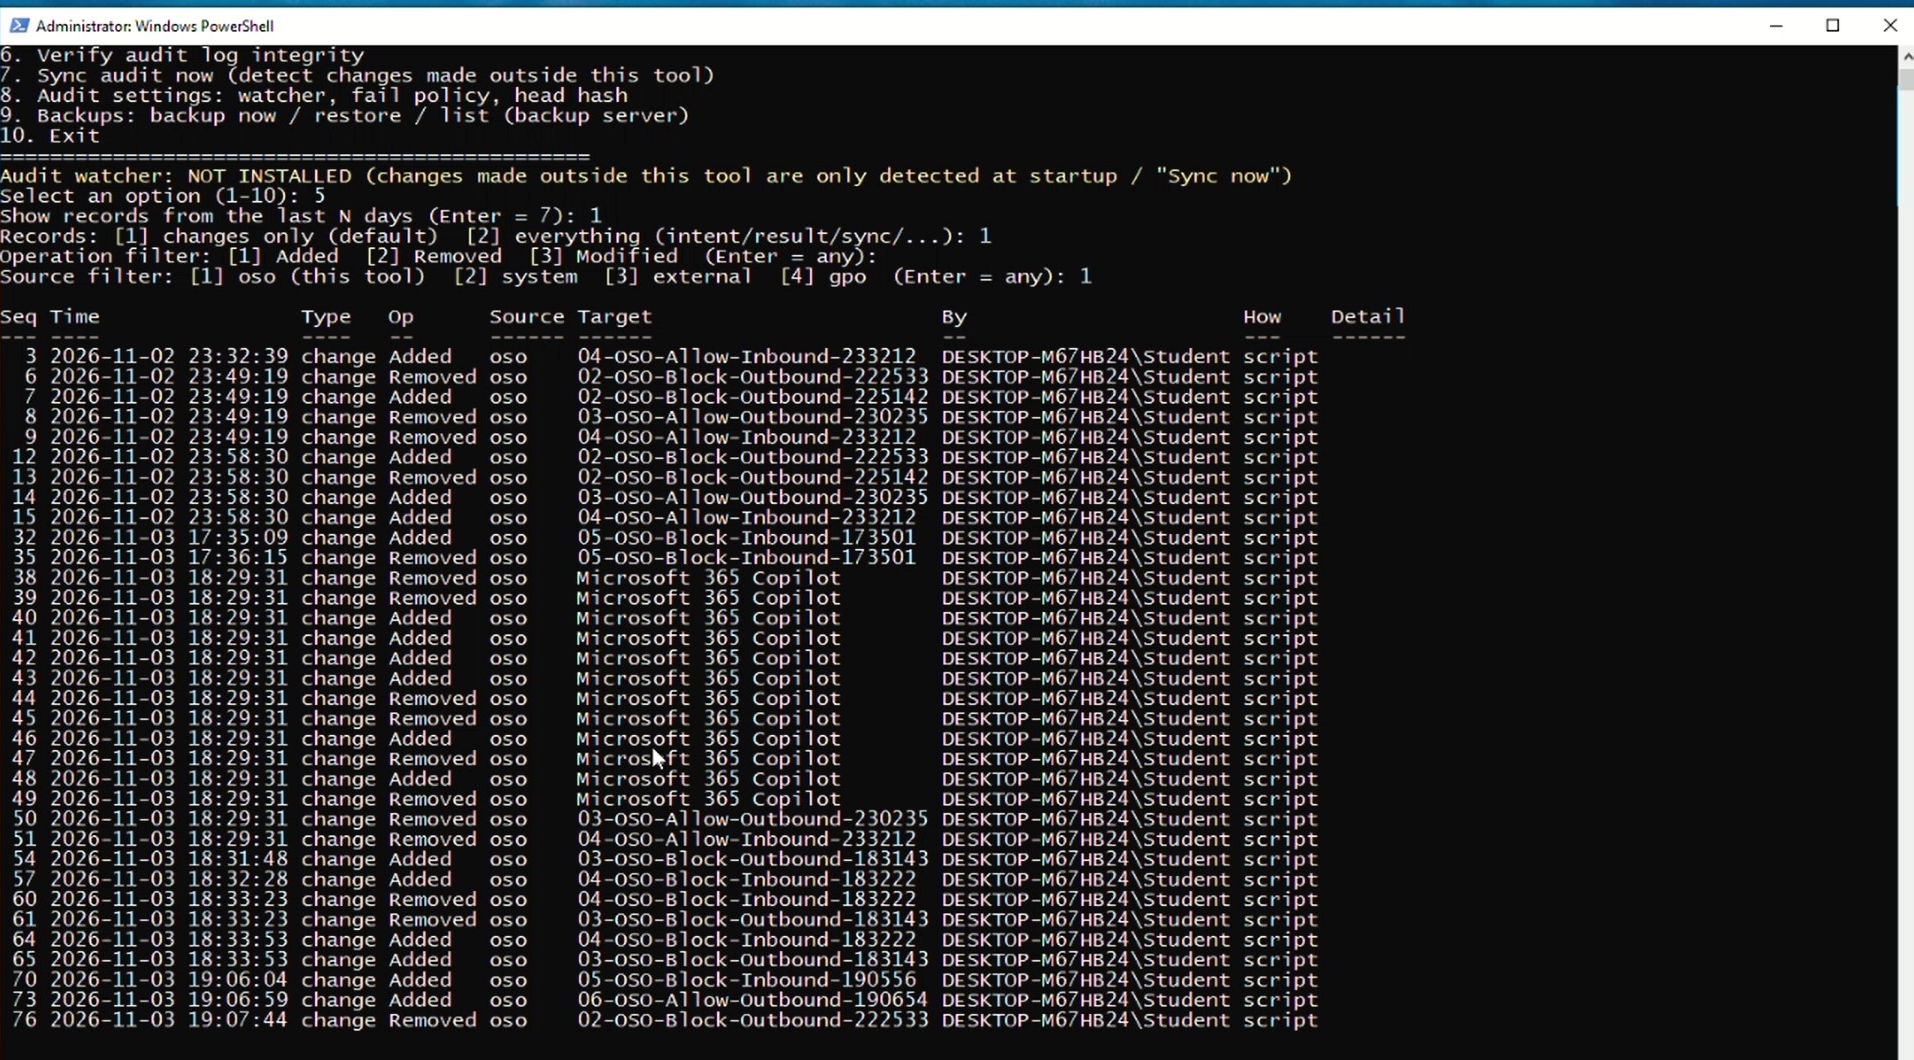
\includegraphics[width=\linewidth, keepaspectratio]{images/audit_log_view.png}
        \caption{Przeglądarka dziennika audytu (opcja menu 5) prezentująca chronologiczną historię zmian polityki wraz z identyfikacją użytkownika i metody detekcji}\label{fig:audit-log-sub1}
    \end{subfigure}\\[6pt]
    \begin{subfigure}[b]{\linewidth}
        \centering
        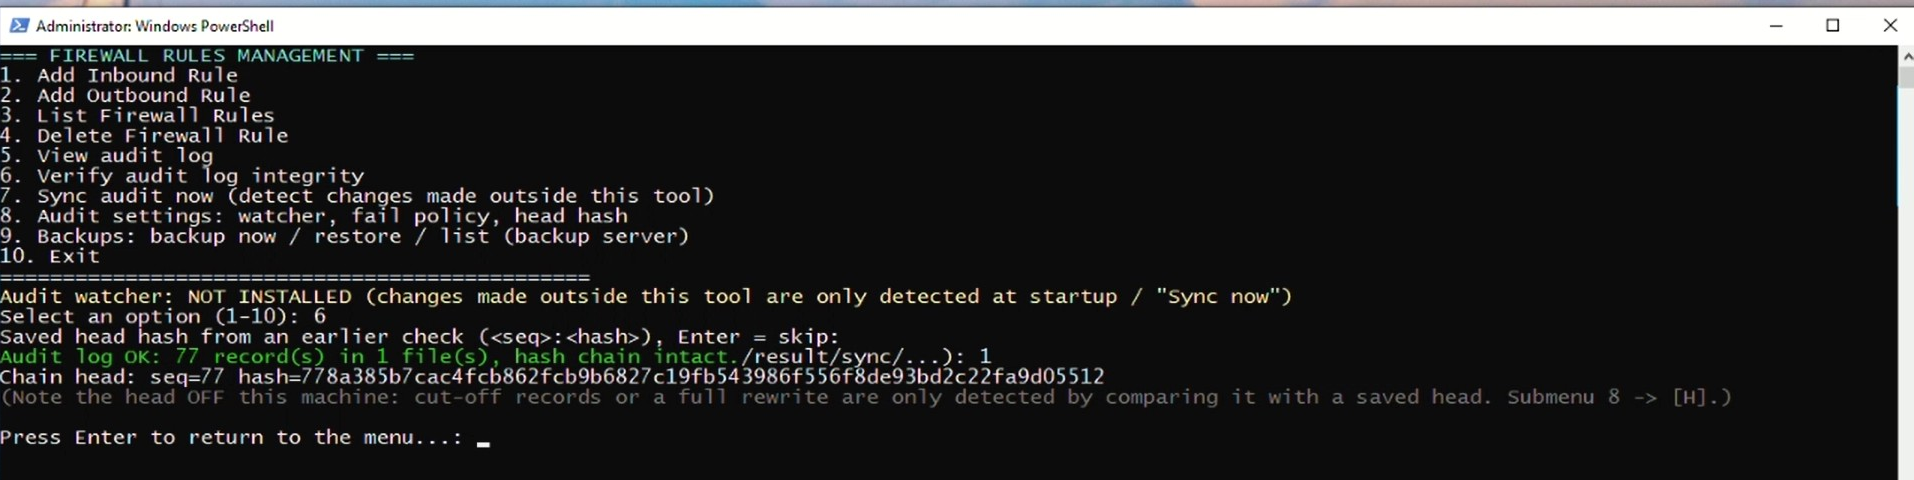
\includegraphics[width=\linewidth, keepaspectratio]{images/audit_integrity.png}
        \caption{Weryfikacja spójności kryptograficznego łańcucha skrótów SHA-256 dziennika audytu (opcja menu 6) wraz z wyznaczeniem bieżącego nagłówka (\textit{Chain head})}\label{fig:audit-integrity}
    \end{subfigure}
    \caption{Interaktywny podgląd historii zmian polityki oraz weryfikacja kryptograficznego łańcucha skrótów SHA-256 w Module 3}\label{fig:audit-log-view}
\end{figure}

\subsection{Wykrywanie zmian zewnętrznych (Watcher) i polityka fail-closed / fail-open}\label{subsec:watcher-i-failpolicy}

Modyfikacje polityki zapory wykonywane poza narzędziem (np.\ w graficznej przystawce \file{wf.msc}, poleceniem \cmd{netsh}, przez silnik zasad grupy GPO lub inny skrypt PowerShell) są przechwytywane przez usługę \textit{Watcher} instalowaną z poziomu podmenu opcji \code{8} (\code{[I] Install / update watcher}, rysunek \ref{fig:audit-watcher-install}). Podczas instalacji skrypt kopiuje sam siebie do izolowanego podkatalogu \file{C:\ProgramData\FirewallAudit\bin\firewall.ps1} zabezpieczonego listą ACL należącą do administratorów i rejestruje zadanie harmonogramu \code{\FirewallAudit\Watcher} uruchamiane na koncie \code{SYSTEM}.

Zadanie \textit{Watcher} jest wyzwalane przez trzy niezależne mechanizmy:
\begin{enumerate}
    \item \textbf{Wyzwalacz zdarzeniowy (\textit{Event Trigger})} - subskrypcja XPath na kanale dziennika zapory reagująca natychmiast na zdarzenia o identyfikatorach \code{2002}-\code{2006}, \code{2033}, \code{2052}, \code{2059} oraz \code{2097}-\code{2099}. Aby uniknąć wielokrotnego wyliczania migawek podczas masowych operacji (np.\ importu polityki generującego setki zdarzeń w ciągu kilku sekund), po uruchomieniu \textit{Watcher} odczekuje na ustabilizowanie licznika \code{RecordId} w dzienniku zdarzeń (brak nowych zdarzeń przez 3 kolejne sekundy, maksymalnie do 30 s), po czym wykonuje pojedynczą synchronizację zbiorczą.
    \item \textbf{Wyzwalacz startowy (\textit{AtStartup})} - weryfikacja stanu polityki podczas rozruchu systemu operacyjnego.
    \item \textbf{Wyzwalacz okresowy (co 15 minut)} - siatka bezpieczeństwa gwarantująca wykrycie zmian zewnętrznych nawet w sytuacji, gdy kanał dziennika zdarzeń zapory został wyłączony przez administratora, przepełniony lub wyczyszczony. Stan zdrowia zadania jest raportowany w pliku \file{state.json} i wyświetlany pod menu głównym (\code{Healthy}, \code{Failed}, \code{Stale} po braku udanego przebiegu przez $>45$ min).
\end{enumerate}

\Figure[1.0]{audit_watcher_install.png}{Podmenu ustawień audytu (opcja 8): diagnostyka dziennika zdarzeń zapory, konfiguracja polityki awarii oraz instalacja zadania systemowego \textit{Watcher}}{fig:audit-watcher-install}

Algorytm synchronizacji stanu polityki, korelacji zmian zewnętrznych z dziennikiem zdarzeń Windows oraz weryfikacji łańcucha skrótów przedstawiono w algorytmie \ref{alg:synchronizacja-i-weryfikacja}.

\begin{algorithm}[H]
    \caption{Synchronizacja stanu polityki zapory, atrybucja zmian zewnętrznych i weryfikacja łańcucha skrótów}\label{alg:synchronizacja-i-weryfikacja}
    \Input{Wyzwalacz $\mathit{Trig} \in \{\texttt{startup}, \texttt{manual}, \texttt{task}\}$, opcjonalny zapamiętany nagłówek łańcucha $\langle s_{\text{exp}}, h_{\text{exp}} \rangle$}
    \Output{Bilans wykrytych zmian zewnętrznych oraz raport integralności łańcucha dziennika}
    \textbf{Część A: Synchronizacja i wykrywanie zmian zewnętrznych (\code{Invoke-AuditSync})}\;
    Pozyskaj muteks \code{Global\FirewallAuditLog}, wczytaj bazę $B$, wykonaj migawkę $S_{\text{now}}$ i wylicz $\Delta \leftarrow \operatorname{CompareSnapshots}(B.\mathit{Entries}, S_{\text{now}})$\;
    Domknij przerwane transakcje (\code{intent} bez \code{result}) statusem \code{recovered} oraz uzgodnij znaczniki z \file{pending.jsonl} (\code{unlogged-change})\;
    \For{każdej różnicy $d \in \Delta$}{
        \lIf{klucz $d.\mathit{Key}$ należy do drzewa GPO}{$\mathit{src} \leftarrow \code{gpo}$; $\mathit{actor} \leftarrow \texttt{unknown (GPO engine)}$}
        \Else{
            Dopasuj zdarzenie z kanału \texttt{Firewall} po $\mathit{RuleId}$ i rozwiąż SID sprawcy $\operatorname{ResolveSid}(\mathit{ModifyingUser})$\;
            \lIf{SID systemowy \textbf{oraz} proces $\in \{\file{svchost.exe}, \file{services.exe}, \file{lsass.exe}\}$}{$\mathit{src} \leftarrow \code{system}$} \lElse{$\mathit{src} \leftarrow \code{external}$}
        }
        $\mathit{det} \leftarrow \text{jeżeli } \mathit{Trig} = \texttt{task} \text{ to } \code{watcher} \text{ w p.p. } \code{reconcile}$\;
        Zapisz rekord $\operatorname{WriteRecord}(\texttt{type}=\code{change}, d, \texttt{source}=\mathit{src}, \texttt{detection}=\mathit{det}, \texttt{actor}=\mathit{actor})$\;
    }
    \lIf{$\Delta \neq \emptyset$ \textbf{lub} odzyskano transakcje \textbf{lub} $\mathit{Trig} = \texttt{manual}$}{zapisz rekord \texttt{sync} z nowym skrótem $h_B$ i zaktualizuj \file{baseline.json}}
    Zwolnij muteks \code{Global\FirewallAuditLog}\;
    \textbf{Część B: Weryfikacja łańcucha skrótów (\code{Test-AuditLogIntegrity})}\;
    $h_{\text{prev}} \leftarrow 0^{64}$; $s_{\text{prev}} \leftarrow 0$; $\mathit{foundHead} \leftarrow \text{fałsz}$\;
    \For{każdego wiersza $L$ w plikach od najstarszego zrotowanego do \file{audit.jsonl}}{
        Wyodrębnij deklarowany skrót $h_{\text{claim}}$ oraz ciało rekordu $J \leftarrow L \setminus \{\code{hash}\}$\;
        \lIf{$\operatorname{SHA256}(J) \neq h_{\text{claim}}$ \textbf{lub} $J.\mathit{prev} \neq h_{\text{prev}}$ \textbf{lub} $J.\mathit{seq} \neq s_{\text{prev}} + 1$}{\textbf{zgłoś błąd} naruszenia ciągłości łańcucha}
        \If{podano $\langle s_{\text{exp}}, h_{\text{exp}} \rangle$ \textbf{oraz} $J.\mathit{seq} = s_{\text{exp}}$}{
            $\mathit{foundHead} \leftarrow \text{prawda}$; \lIf{$h_{\text{claim}} \neq h_{\text{exp}}$}{\textbf{zgłoś błąd} przepisania dziennika względem \textit{head hash}}
        }
        $h_{\text{prev}} \leftarrow h_{\text{claim}}$; $s_{\text{prev}} \leftarrow J.\mathit{seq}$\;
    }
    \lIf{podano $\langle s_{\text{exp}}, h_{\text{exp}} \rangle$ \textbf{oraz} $\mathit{foundHead} = \text{fałsz}$}{\textbf{zgłoś błąd} obcięcia końca dziennika}
    \Return{Raport spójności łańcucha oraz bilans synchronizacji}\;
\end{algorithm}

Moduł implementuje ponadto jawny mechanizm sterowania polityką reakcji na awarię dziennika (\textit{fail-closed} vs \textit{fail-open}):
\begin{itemize}
    \item \textbf{Tryb \code{Closed} (domyślny)} - nadrzędność rozliczalności: jeżeli dziennik audytu jest zablokowany przez inny proces po upływie czasu oczekiwania (60 s), uszkodzony lub katalog audytu ma nieprawidłowego właściciela, żadna zmiana polityki zapory nie zostaje wykonana.
    \item \textbf{Tryb \code{Open} (awaryjny)} - umożliwia wykonanie zmiany w sytuacji awarii dziennika, jednak zmiana trybu na \code{Open} wymaga podania powodu i zapisania wyprzedzającego rekordu \code{setting} w samym dzienniku audytu wraz ze skrótem pliku \file{settings.json}. Ręczna edycja pliku \file{settings.json} w notatniku w celu cichego wyłączenia blokady jest wykrywana przy starcie (skrót w pliku nie zgadza się z ostatnim rekordem \code{setting} w dzienniku), co automatycznie wymusza powrót do trybu \code{Closed} i rejestruje incydent \code{settings-file-modified}. Ponadto aktywny tryb \code{Open} wyświetla w menu głównym czerwony baner ostrzegawczy \code{AUDIT FAIL-OPEN}, a każda wykonana w tym czasie zmiana odkłada znacznik w pliku \file{pending.jsonl} (lub w systemowym dzienniku zdarzeń \code{Application} o ID \code{4001}).
\end{itemize}

\section{Moduł 4: Zdalne kopie zapasowe i odtwarzanie polityki}\label{sec:modul-backup}

Czwarty moduł funkcjonalny (autor: Ruslan Hedz) odpowiada za automatyczne oraz ręczne tworzenie kopii zapasowych pełnej polityki zapory na zewnętrznym serwerze Ubuntu (\code{10.0.2.30}), ich inwentaryzację oraz bezpieczne przywracanie na stacji roboczej Windows (\code{10.0.2.20}).

\subsection{Architektura komunikacji klient-serwer i protokół eksportu (pull)}\label{subsec:eksport-konfiguracji}

Aby uniemożliwić stacji klienckiej nadpisywanie lub kasowanie historycznych kopii zapasowych na serwerze, proces tworzenia kopii realizowany jest w architekturze odwróconego pobierania (\textit{server-side pull}):

\begin{enumerate}
    \item \textbf{Inicjacja kopii przez klienta} - stacja Windows (automatycznie przed modyfikacją reguł lub ręcznie w podmenu kopii) nawiązuje połączenie SSH z kontem \code{fwbackup@10.0.2.30} na porcie 22, przekazując polecenie \textbf{backup <powód>} (ze zdefiniowaną listą dopuszczalnych powodów: \code{manual}, \code{auto-add}, \code{auto-delete}, \code{pre-restore} lub \code{scheduled}).
    \item \textbf{Weryfikacja i blokada na serwerze} - demon \code{sshd} na serwerze Ubuntu ignoruje oryginalne polecenie powłoki i na podstawie dyrektywy wymuszonego polecenia (\code{command=...}) w pliku \file{authorized_keys} uruchamia skrypt \file{fw-server.sh} ze sztywno przypisaną tożsamością klienta. Skrypt sprawdza klienta w pliku \file{/etc/fwbackup/clients.conf} (nie ufając argumentom) i zakłada blokadę \cmd{flock}.
    \item \textbf{Pobranie polityki przez serwer (Agent Export)} - serwer Ubuntu nawiązuje połączenie zwrotne SSH na port 22 stacji Windows przy użyciu klucza prywatnego \file{/etc/fwbackup/id_export} (do 3 prób). Na stacji Windows klucz ten w pliku \file{administrators_authorized_keys} ma zablokowane powłoki i tunele (\code{restrict}) i wymusza uruchomienie wyłącznie agenta eksportu:
    \begin{center}
        \code{powershell.exe -NoProfile -ExecutionPolicy Bypass -File C:/FW/FirewallRules.ps1 -Agent Export}
    \end{center}
    Agent eksportuje politykę poleceniem \cmd{netsh.exe advfirewall export} do chronionego katalogu tymczasowego, oblicza skrót SHA-256 i zwraca przez strumień \code{stdout} ustrukturyzowaną odpowiedź: nagłówek \code{FWAGENT-BEGIN}, pola \code{COMPUTER=<nazwa>}, \code{SHA256=<hash>}, \code{SIZE=<bajty>}, blok \code{DATA} z zawartością pliku \file{.wfw} zakodowaną w Base64 oraz stopkę \code{FWAGENT-END}.
    \item \textbf{Weryfikacja i zapis na serwerze} - skrypt \file{fw-server.sh} dekoduje strumień Base64, oblicza niezależnie skrót SHA-256 odebranego pliku binarnego i porównuje go z wartością zadeklarowaną przez agenta. W przypadku zgodności zapisuje kopię w katalogu \file{/srv/fwbackups/<user>/backups/} pod nazwą:
    \[
        \texttt{<KOMPUTER>\_<YYYYMMDD>\_<HHMMSS>\_<powód>.wfw}
    \]
    oraz bliźniaczy plik sumy kontrolnej \file{.wfw.sha256}. Zapis wykonywany jest do plików tymczasowych \file{.part} z zamianą (\cmd{mv -f}) oraz dziedziczeniem grupy \code{sftpgo} (bit \code{setgid} \code{2750} na katalogu), przy czym plik \file{.sha256} tworzony jest jako ostatni - dzięki temu klient listujący katalog przez SFTP widzi wyłącznie kompletne, zweryfikowane kopie. Na końcu serwer wykonuje retencję (\code{prune}), zachowując 30 najnowszych kopii automatycznych (\code{auto-*} oraz \code{scheduled}), nigdy nie usuwając kopii manualnych ani kopii aktualnie odtwarzanej.
\end{enumerate}

\subsection{Dwufazowa procedura odtwarzania polityki (Restore) i weryfikacja spójności}\label{subsec:import-konfiguracji}

Odtwarzanie polityki zapory (opcja menu \code{9} $\rightarrow$ \code{[R]}) zostało zaprojektowane tak, aby serwer kopii nie posiadał uprawnień do zdalnego wgrywania polityki na stację Windows (eliminuje to ryzyko przejęcia stacji roboczych w przypadku kompromitacji serwera kopii oraz rozwiązuje problem blokowania potoków wejściowych SSH):

\begin{enumerate}
    \item \textbf{Inwentaryzacja i wybór kopii} - klient łączy się przez protokół SFTP z serwerem SFTPGo na porcie 2022, pobiera listę plików z wirtualnego katalogu \file{backups/}, filtruje wyłącznie wpisy posiadające parę \file{.wfw} + \file{.wfw.sha256} i wyświetla tabelę zawierającą indeks, datę, powód utworzenia oraz nazwę pliku (rysunek \ref{fig:backup-restore}).
    \item \textbf{Faza I (Przygotowanie na serwerze i kopia ratunkowa \code{pre-restore})} - po wybraniu numeru kopii, podaniu decyzji o utworzeniu kopii ratunkowej bieżącego stanu (domyślnie \code{yes}) oraz wpisaniu słowa potwierdzającego \code{RESTORE}, klient wysyła do serwera po SSH rozkaz \code{restore <plik.wfw> <yes|no>}. Serwer oznacza wskazaną kopię jako chronioną przed retencją (\code{PROTECT}), sprawdza jej integralność SHA-256 na dysku serwera, wykonuje kopię ratunkową bieżącej polityki z powodem \code{pre-restore}, ponownie weryfikuje plik docelowy i zwraca potwierdzenie \code{STATUS=OK}.
    \item \textbf{Faza II (Pobranie po SFTP, weryfikacja lokalna i zaudytowany import)} - po otrzymaniu potwierdzenia z serwera stacja Windows pobiera plik \file{<plik>.wfw} oraz \file{<plik>.wfw.sha256} przez SFTPGo (korzystając z uprawnień tylko do odczytu \code{list} + \code{download}), wylicza lokalnie skrót SHA-256 pobranego pliku i porównuje go ze skrótem z pliku \file{.sha256}. Dopiero po pozytywnej weryfikacji kryptograficznej wywoływany jest transakcyjny mechanizm audytu (\code{Operation = 'Restore'}, \code{Scope = 'All'}), wewnątrz którego wykonywany jest import \cmd{netsh.exe advfirewall import} oraz natychmiastowe wywołanie procedury \code{EnsureSshRule()}. Ponieważ odtwarzanie jest inicjowane bezpośrednio z lokalnej konsoli administratora, import starszej polityki pozbawionej reguły \code{FWBackup-SSH-In} nie przerywa sesji konsolowej, a reguła dostępowa dla serwera kopii zostaje odtworzona zanim system obsłuży jakiekolwiek nowe pakiety sieciowe.
\end{enumerate}

Przebieg procedury wyboru kopii, wykonania zrzutu ratunkowego \code{pre-restore} i przywrócenia polityki oraz zaktualizowaną listę kopii na serwerze przedstawiono na rysunku \ref{fig:backup-restore}.

\begin{figure}[H]
    \centering
    \begin{subfigure}[b]{\linewidth}
        \centering
        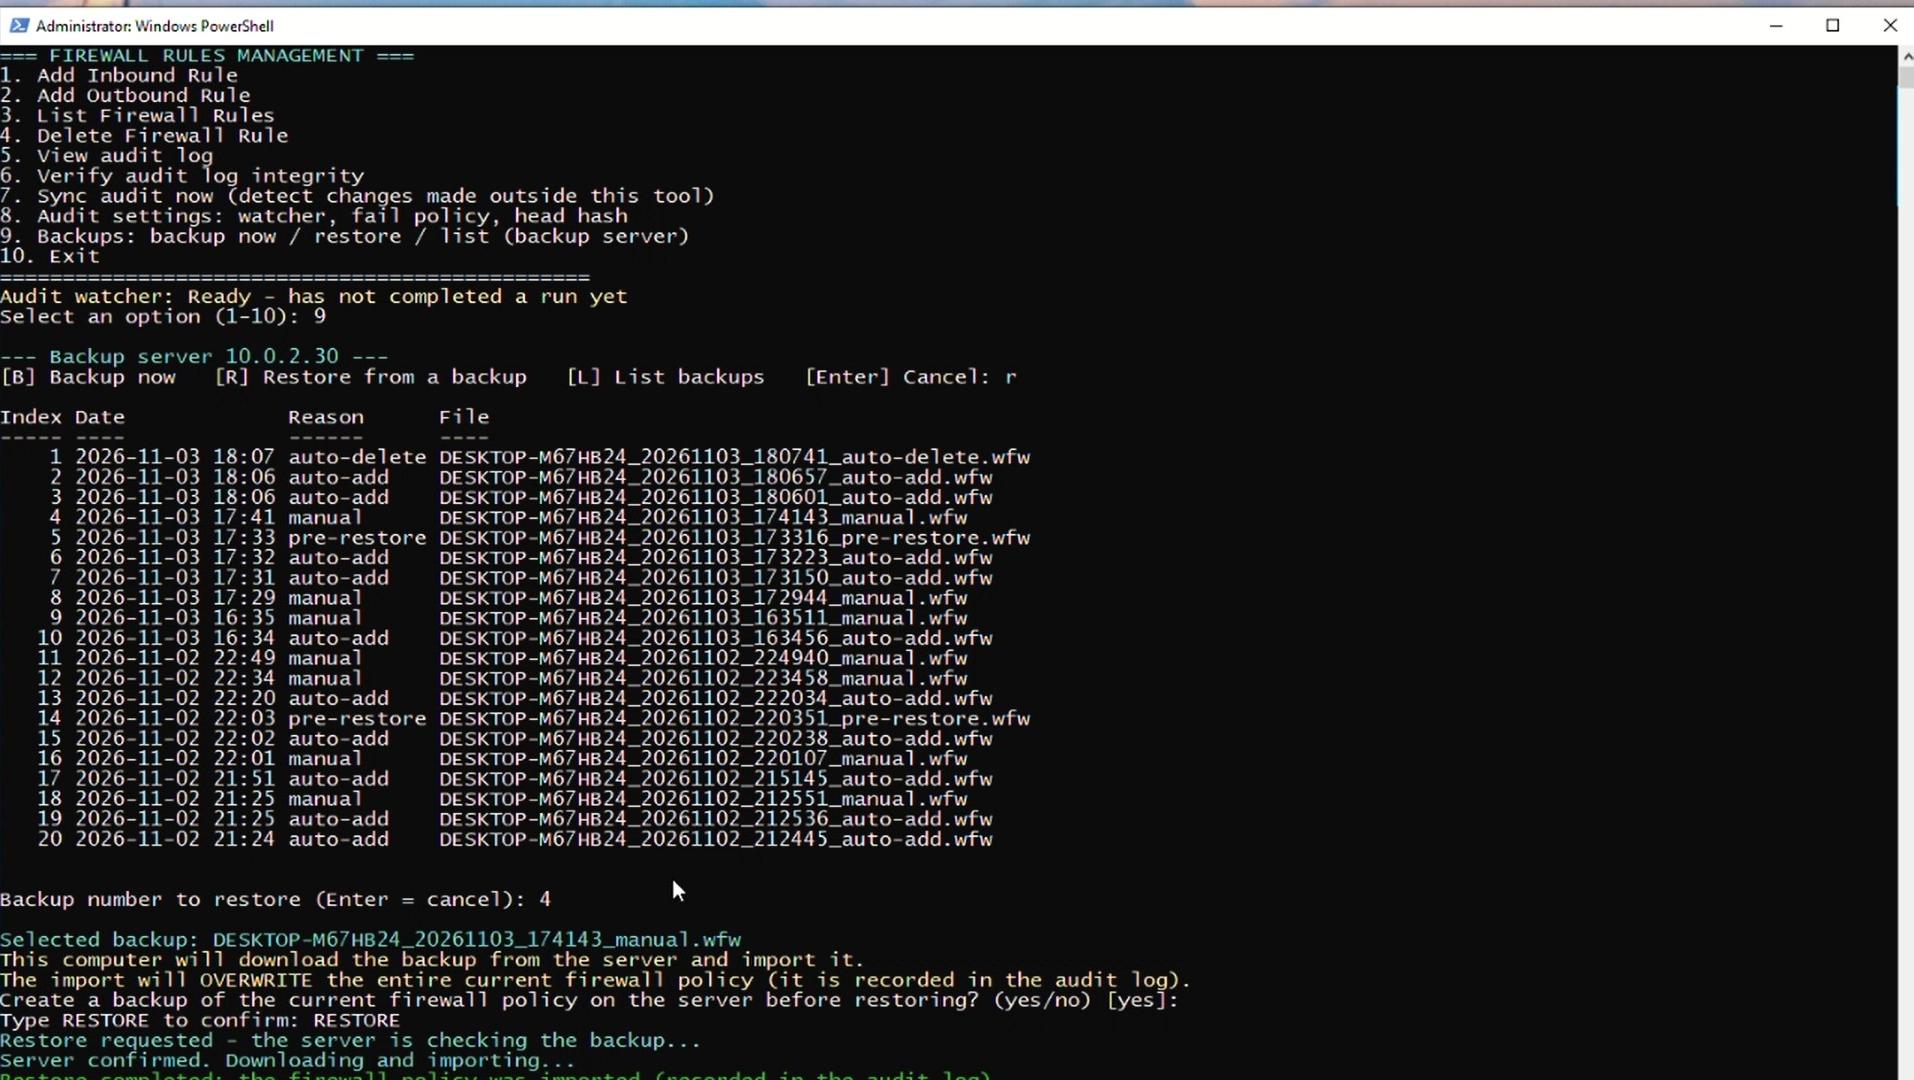
\includegraphics[width=\linewidth, keepaspectratio]{images/backup_restore.png}
        \caption{Procedura przywracania polityki zapory (opcja menu 9 $\rightarrow$ R) z utworzeniem kopii ratunkowej \code{pre-restore} i potwierdzeniem \code{RESTORE}}\label{fig:backup-restore-sub1}
    \end{subfigure}\\[6pt]
    \begin{subfigure}[b]{\linewidth}
        \centering
        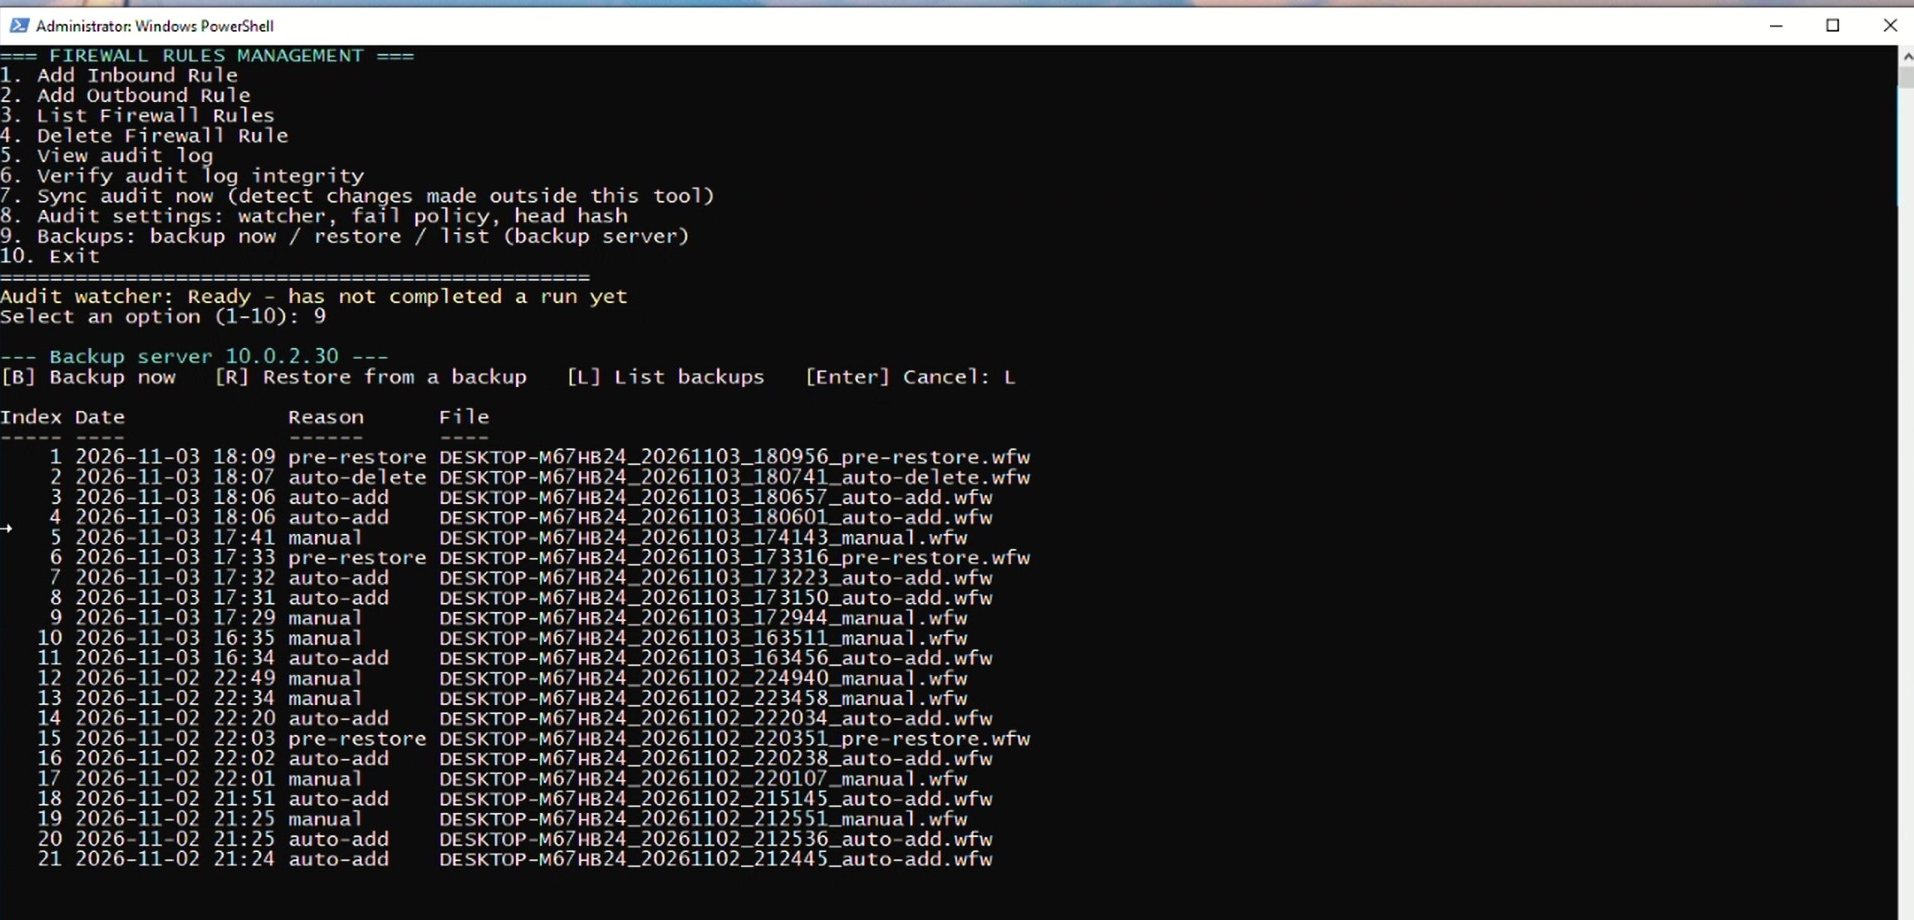
\includegraphics[width=\linewidth, keepaspectratio]{images/backup_list.png}
        \caption{Lista kopii zapasowych na serwerze \code{10.0.2.30} po zakończeniu odtwarzania, uwzględniająca nowo utworzoną kopię \code{pre-restore}}\label{fig:backup-list}
    \end{subfigure}
    \caption{Dwufazowe odtwarzanie polityki zapory z serwera zdalnego oraz inwentaryzacja kopii przez kanał SFTPGo w Module 4}\label{fig:backup-restore}
\end{figure}

Formalny zapis algorytmu tworzenia kopii w modelu \textit{pull} oraz dwufazowego odtwarzania konfiguracji przedstawiono w algorytmie \ref{alg:backup-i-restore}.

\begin{algorithm}[H]
    \caption{Zdalne tworzenie kopii zapasowej w modelu \textit{pull} oraz dwufazowe odtwarzanie polityki zapory}\label{alg:backup-i-restore}
    \Input{Tryb $M \in \{\texttt{Backup}, \texttt{Restore}\}$, powód $\mathit{Reason}$ lub plik kopii $F_{\text{target}}$ i flaga $\mathit{Pre} \in \{\texttt{yes}, \texttt{no}\}$}
    \Output{Status operacji kopii zapasowej lub zaudytowanego odtworzenia polityki zapory}
    \If{$M = \texttt{Backup}$}{
        Klient wysyła po SSH (port 22, wymuszone polecenie) żądanie $\code{backup } \parallel \mathit{Reason}$; serwer zakłada blokadę \cmd{flock}\;
        Serwer łączy się zwrotnie po SSH (klucz \file{id_export}) ze stacją Windows, wywołując \code{-Agent Export}\;
        Agent weryfikuje regułę \texttt{FWBackup-SSH-In}, wykonuje \cmd{netsh advfirewall export} do pliku $T$, wylicza $h_{\text{win}} \leftarrow \operatorname{SHA256}(T)$ i zwraca $\operatorname{Base64}(T)$\;
        Serwer dekoduje strumień do pliku $T_{\text{srv}}$ i wylicza $h_{\text{srv}} \leftarrow \operatorname{SHA256}(T_{\text{srv}})$\;
        \lIf{$T_{\text{srv}}$ jest pusty \textbf{lub} $h_{\text{srv}} \neq h_{\text{win}}$}{\Return{\texttt{FAIL: niezgodność sumy kontrolnej SHA-256 lub błąd eksportu}}}
        Zapisz atomowo $\mathit{Name}.\file{wfw}$ oraz $\mathit{Name}.\file{wfw.sha256}$ (grupa \texttt{sftpgo}, prawa \texttt{0640}) i usuń nadmiarowe kopie ponad $\mathit{KEEP\_AUTO} = 30$\;
        \Return{$\texttt{OK: } \mathit{Name}.\file{wfw}$}\;
    }
    \ElseIf{$M = \texttt{Restore}$}{
        Klient pobiera przez SFTPGo (port 2022) listę par $\file{*.wfw} + \file{*.wfw.sha256}$; po wpisaniu \texttt{RESTORE} wysyła po SSH $\code{restore } \parallel F_{\text{target}} \parallel \text{\code{ }} \parallel \mathit{Pre}$\;
        Serwer oznacza $F_{\text{target}}$ jako chroniony ($\mathit{PROTECT}$) i weryfikuje jego skrót SHA-256 na dysku\;
        \If{$\mathit{Pre} = \texttt{yes}$}{
            Serwer wykonuje kopię ratunkową z powodem $\code{pre-restore}$; \lIf{błąd kopii}{\Return{\texttt{FAIL: przerwano przed nadpisaniem polityki}}}
        }
        Klient pobiera przez SFTPGo pliki $F_{\text{target}}$ i $F_{\text{target}}.\file{sha256}$, wylicza lokalnie $h_{\text{calc}} \leftarrow \operatorname{SHA256}(F_{\text{target}})$ i porównuje z $h_{\text{exp}}$\;
        \lIf{$h_{\text{calc}} \neq h_{\text{exp}}$}{usuń pliki tymczasowe i \textbf{zgłoś wyjątek} \enquote{Niezgodność SHA-256 pobranej kopii - import zablokowany}}
        Wykonaj $\operatorname{AuditedChange}\bigl(\texttt{Operation}=\code{Restore},\; \texttt{Scope}=\texttt{All},\; \texttt{Action}=\{\cmd{netsh advfirewall import } F_{\text{target}};\; \operatorname{EnsureSshRule}()\}\bigr)$\;
        Usuń pliki tymczasowe i \Return{\texttt{OK: polityka przywrócona i zarejestrowana w audycie}}\;
    }
\end{algorithm}

\chapter{Środowisko uruchomieniowe i weryfikacja działania}\label{ch:testy}

Niniejszy rozdział charakteryzuje środowisko uruchomieniowe wykorzystane do wdrożenia systemu oraz przedstawia metodykę i wyniki weryfikacji działania poszczególnych modułów, obejmującej automatyczny potok CI/CD, izolowane testy jednostkowe w piaskownicy oraz uprzywilejowane testy akceptacyjne.

\section{Środowisko uruchomieniowe i konfiguracja bezpieczeństwa}\label{sec:srodowisko-testowe}

System został wdrożony i przetestowany w dwuwęzłowej architekturze sieciowej łączącej zarządzaną stację roboczą z systemem Microsoft Windows oraz dedykowany serwer kopii zapasowych z systemem Linux. Parametry obu węzłów oraz skonfigurowanych usług zestawiono w tabeli~\ref{tab:srodowisko-testowe}, natomiast całościową topologię połączeń, komponentów i przepływów protokołów komunikacyjnych przedstawiono na rysunku~\ref{fig:environment-topology}.

\Figure[1.0]{environment_topology.png}{Topologia dwuwęzłowego środowiska uruchomieniowego, separacja ról oraz kierunki przepływu protokołów komunikacyjnych}{fig:environment-topology}

\begin{table}[H]
    \centering
    \caption{Konfiguracja węzłów środowiska uruchomieniowego i testowego}\label{tab:srodowisko-testowe}
    \tablefont
    \begin{tabularx}{\linewidth}{L{3.2cm} L{5.4cm} Y}
        \toprule
        \hcell{Parametr} & \hcell{Stacja robocza (Klient)} & \hcell{Serwer kopii zapasowych} \\
        \midrule
        System operacyjny & Microsoft Windows 10 Pro & Ubuntu Linux 26.04 LTS \\
        Adresacja IP (LAN) & \code{10.0.2.20} & \code{10.0.2.30} \\
        Środowisko skryptowe & Windows PowerShell 5.1 (\textit{Desktop Edition}), .NET 4.8 & Powłoka systemowa \cmd{bash}, narzędzia \cmd{flock}, \cmd{sha256sum}, \cmd{base64} \\
        Usługi komunikacyjne & OpenSSH Client + OpenSSH Server (\code{sshd} na porcie TCP 22) & OpenSSH Server (port TCP 22) + SFTPGo (port TCP 2022) \\
        Konta operacyjne & Konto administratora \code{Student} + konto \code{SYSTEM} (\textit{Watcher}) & Konto systemowe \code{fwbackup} + konto usługi \code{sftpgo} \\
        Katalogi chronione & \file{C:\FW}, \file{C:\ProgramData\FirewallAudit}, \file{C:\ProgramData\FirewallBackup} & \file{/etc/fwbackup}, \file{/srv/fwbackups/student/backups} \\
        \bottomrule
    \end{tabularx}
\end{table}

W celu zapewnienia odporności wdrożenia na lokalną eskalację uprawnień oraz nieautoryzowany dostęp sieciowy zastosowano następujące środki utwardzania konfiguracji:
\begin{enumerate}
    \item \textbf{Ochrona katalogów skryptów i dzienników na stacji Windows} - katalogi \file{C:\FW} oraz \file{C:\ProgramData\FirewallAudit} posiadają wyłączone dziedziczenie uprawnień DACL (\cmd{icacls.exe /inheritance:r}) i przyznają prawa zapisu wyłącznie kontom \code{SYSTEM} (\code{S-1-5-18}) oraz \code{Administratorzy} (\code{S-1-5-32-544}). Przed załadowaniem modułów \file{Backup-Create.ps1} i \file{Backup-Restore.ps1} skrypt główny weryfikuje listę ACL i odmawia uruchomienia w przypadku wykrycia praw zapisu dla nieuprzywilejowanych kont.
    \item \textbf{Restrykcje usługi OpenSSH na stacji Windows} - w pliku konfiguracyjnym \file{sshd_config} ograniczono dostęp dyrektywami \code{AllowUsers student@10.0.2.30} oraz \code{PasswordAuthentication no}, a reguła zapory \code{FWBackup-SSH-In} zezwala na ruch przychodzący na port TCP~22 wyłącznie ze wskazanego adresu IP serwera kopii (\code{10.0.2.30}).
    \item \textbf{Separacja uprawnień na serwerze Ubuntu} - skrypt \file{fw-server.sh} należy do konta \code{root} (\code{0755}), katalog kopii \file{/srv/fwbackups/student/backups} posiada uprawnienia \code{2750} (\code{fwbackup:sftpgo}, bit \code{setgid}), a wirtualne konto \code{student} w SFTPGo ma przyznane wyłącznie uprawnienia \code{list} oraz \code{download}.
\end{enumerate}

\section{Weryfikacja funkcjonalna i testy automatyczne}\label{sec:testy-weryfikacja}

Strategię weryfikacji poprawności działania systemu podzielono na trzy uzupełniające się poziomy: zautomatyzowaną analizę statyczną w potoku CI/CD, izolowane testy jednostkowe w piaskownicy (wykonywane bez uprawnień administratora) oraz rzeczywiste testy akceptacyjne na dedykowanej maszynie wirtualnej.

\subsection{Automatyczny potok CI/CD i analiza statyczna kodu}\label{subsec:potok-ci-cd}

W repozytorium kodu wdrożono zautomatyzowany potok CI/CD oparty na GitHub Actions (\file{.github/workflows/ci.yml}), który przy każdym commicie oraz żądaniu pull request uruchamia dwa równoległe zadania weryfikacyjne:
\begin{itemize}
    \item \textbf{Środowisko Windows (\code{windows-latest})} - weryfikuje poprawność składniową kodu PowerShell za pomocą lintera \code{PSScriptAnalyzer} (z rygorystycznym filtrem \code{-Severity Error}), po czym uruchamia testy jednostkowe modułu audytu, interfejsu CLI oraz modułu kopii zapasowych.
    \item \textbf{Środowisko Linux (\code{ubuntu-latest})} - wykonuje analizę statyczną skryptu powłoki serwera \file{fw-server.sh} narzędziem \cmd{shellcheck} (weryfikacja błędów składniowych i podatności w skryptach powłoki), a następnie uruchamia zestaw testów jednostkowych serwera w środowisku \cmd{bash}.
\end{itemize}

Dzięki takiemu podejściu wszelkie regresje składniowe lub naruszenia kontraktów API są natychmiast wychwytywane przed scaleniem zmian.

\subsection{Izolowane testy jednostkowe w piaskownicy (\file{tests/})}\label{subsec:testy-jednostkowe}

Aby umożliwić szybką weryfikację logiki aplikacji na stacjach deweloperskich oraz w kontenerach CI/CD bez konieczności podnoszenia uprawnień do poziomu administratora i bez ingerencji w rzeczywiste reguły sieciowe jądra, opracowano zestaw testów jednostkowych działających w bezpiecznej piaskownicy (\textit{sandbox}):
\begin{enumerate}
    \item \textbf{Audyt transakcyjny i kontrakt AST (\file{Test-FirewallAudit.ps1})} - przekierowuje operacje rejestru do gałęzi \code{HKCU\Software\FwAuditTest-<GUID>}, wykorzystuje lokalny muteks oraz tymczasowy katalog w \file{\%TEMP\%}. Sprawdza integralność łańcucha skrótów SHA-256, procedurę rotacji przy 10~MB oraz politykę \textit{fail-closed}/\textit{fail-open}. Ponadto za pomocą analizatora AST (\code{Language.Parser}) bada cały plik \file{firewall.ps1}, weryfikując, czy wszystkie modyfikacje zapory (cmdlety \cmd{*-NetFirewallRule} i program \cmd{netsh advfirewall}) są hermetycznie opakowane w wywołanie \code{Invoke-AuditedChange}.
    \item \textbf{Interfejs CLI i walidacja danych (\file{Test-CliHelpers.ps1})} - wyodrębnia za pomocą AST funkcje pomocnicze (\code{Read-ProfileChoice}, \code{Read-ProtocolChoice}, \code{Get-AuditPolicyStatusLine}) i testuje je z wykorzystaniem deterministycznej kolejki wejściowej mockującej polecenie \cmd{Read-Host}. Weryfikuje odrzucanie niepoprawnych adresów IPv4/IPv6, masek CIDR i portów spoza zakresu $1\text{-}65535$, automatyczne kierunkowe przypisanie portów oraz format generowanych nazw reguł z prefiksem \code{OSO-}.
    \item \textbf{Klient kopii zapasowych (\file{Test-BackupModule.ps1})} - testuje funkcje modułów \file{Backup-Create.ps1} i \file{Backup-Restore.ps1}. Weryfikuje walidację nazw kont użytkowników wyrażeniem regularnym \code{^[a-z0-9][a-z0-9._-]{0,31}$}, odporność na próby obejścia katalogu (\textit{path traversal}, np.\ \code{../}), obsługę portów SSH/SFTP oraz weryfikację sum kontrolnych SHA-256 pobranych plików polityki \file{.wfw}.
    \item \textbf{Serwer kopii zapasowych Ubuntu (\file{test-fw-server.sh})} - uruchamia wyizolowane procedury skryptu \file{fw-server.sh} w katalogu tymczasowym. Weryfikuje parsowanie pliku konfiguracyjnego \file{clients.conf}, mechanizm blokady współbieżności (\cmd{flock}) oraz politykę retencji archiwum (automatyczne przycinanie najstarszych kopii z zachowaniem maksymalnie 30 ostatnich stanów).
\end{enumerate}

\subsection{Test akceptacyjny end-to-end na maszynie wirtualnej (\file{Invoke-WatcherAcceptance.ps1})}\label{subsec:testy-akceptacyjne}

Weryfikację elementów wymagających rzeczywistych uprawnień administratora oraz interakcji z podsystemami jądra Windows (zadanie harmonogramu \code{SYSTEM}, chroniona lista ACL w \file{C:\ProgramData\FirewallAudit}, odczyt zdarzeń z kanału \code{MPSSVC}) realizuje skrypt akceptacyjny \file{tests\Invoke-WatcherAcceptance.ps1}. Skrypt ten przeprowadza pełny cykl życia systemu na rzeczywistej maszynie wirtualnej:
\begin{enumerate}
    \item weryfikuje ochronę ACL katalogu audytu (brak praw modyfikacji dla grup \code{Users}, \code{Everyone} oraz \code{Authenticated Users}),
    \item instaluje zadanie \code{\FirewallAudit\Watcher} i potwierdza konfigurację 3 wyzwalaczy (zdarzeniowy, startowy, okresowy co 15~min) oraz zgodność skrótu SHA-256 skryptu w katalogu \file{bin},
    \item tworzy i usuwa testową regułę \code{FWAUDIT-ACCEPT-<id>-external} bezpośrednim wywołaniem cmdletu \cmd{New-NetFirewallRule} (poza narzędziem), po czym potwierdza przechwycenie zdarzenia przez zadanie \textit{Watcher} oraz poprawną atrybucję sprawcy z dziennika zdarzeń zapory,
    \item symuluje awarię dziennika poprzez zablokowanie pliku \file{audit.jsonl} wyłącznym uchwytem \code{FileShare.None}, weryfikując zablokowanie zmiany w trybie \code{Closed} oraz prawidłowe odłożenie znacznika i późniejsze uzgodnienie (\textit{reconcile}) w trybie \code{Open},
    \item sprawdza ciągłość łańcucha skrótów SHA-256 i usuwa reguły testowe.
\end{enumerate}

Zbiorcze zestawienie zrealizowanych scenariuszy weryfikacyjnych przedstawiono w tabeli~\ref{tab:wyniki-testow}.

\begin{table}[H]
    \centering
    \caption{Zestawienie scenariuszy weryfikacyjnych i wyników testów wszystkich modułów systemu}\label{tab:wyniki-testow}
    \tablefont
    \begin{tabularx}{\linewidth}{C{1.4cm} L{3.6cm} Y C{1.6cm}}
        \toprule
        \hcell{ID} & \hcell{Badany obszar (Moduł)} & \hcell{Opis scenariusza testowego i kryterium akceptacji} & \hcell{Wynik} \\
        \midrule
        \code{T-01} & Walidacja i numeracja (Moduł 1, \code{WF-01}, \code{WF-02}) & Odrzucanie błędnych adresów IP (ciągi znaków, pojedyncze liczby, oktety $>255$) oraz portów spoza zakresu $1\text{-}65535$; poprawne nadanie numerów \code{05-OSO-*} i \code{06-OSO-*} oraz usuwanie po indeksie. & \cmark \\
        \code{T-02} & Semantyka portów (Moduł 1, \code{WF-01}) & Wymuszenie protokołu TCP/UDP po podaniu portu oraz automatyczne przypisanie \code{LocalPort} dla \textit{Inbound} i \code{RemotePort} dla \textit{Outbound}. & \cmark \\
        \code{T-03} & Profile sieciowe NLA (Moduł 2, \code{WF-03}) & Odczyt aktywnej kategorii interfejsu (\code{Private} na karcie \code{Ethernet}), przypisanie reguł do wybranych profili (\code{Public}, \code{Any}) i ich selektywne egzekwowanie. & \cmark \\
        \code{T-04} & Kontrakt AST i WAL (Moduł 3, \code{WF-04}, \code{WNF-04}) & Analiza statyczna AST pliku \file{firewall.ps1} (brak niezaudytowanych wywołań), trójfazowy zapis \code{intent} $\rightarrow$ \code{change} $\rightarrow$ \code{result}, detekcja \code{scope-escape} i czas migawki $<1$~s. & \cmark \\
        \code{T-05} & Łańcuch skrótów SHA-256 (Moduł 3, \code{WF-06}) & Weryfikacja spójności 77 rekordów w \file{audit.jsonl} oraz wykrycie modyfikacji treści, usunięcia wiersza, obcięcia końca pliku (\textit{head hash}) i podmiany \file{baseline.json}. & \cmark \\
        \code{T-06} & Zadanie \textit{Watcher} (Moduł 3, \code{WF-05}, \code{WNF-02}) & Utworzenie i usunięcie reguły poza narzędziem; przechwycenie zmiany przez zadanie \code{SYSTEM}, atrybucja sprawcy (\code{DESKTOP-M67HB24\Student}) i weryfikacja uprawnień ACL. & \cmark \\
        \code{T-07} & Polityka awarii (Moduł 3, \code{WNF-01}) & Zablokowanie pliku \file{audit.jsonl}: odmowa zmiany w trybie \code{Closed}, wykrycie ręcznej edycji \file{settings.json} oraz uzgodnienie \file{pending.jsonl} w trybie \code{Open}. & \cmark \\
        \code{T-08} & Eksport \textit{pull} (Moduł 4, \code{WF-07}, \code{WNF-03}) & Automatyczne utworzenie kopii na serwerze \code{10.0.2.30} przed dodaniem (\code{auto-add}) i usunięciem reguły (\code{auto-delete}); weryfikacja sumy SHA-256 i grup SFTPGo. & \cmark \\
        \code{T-09} & Odtwarzanie polityki (Moduł 4, \code{WF-08}, \code{WNF-03}) & Przywrócenie kopii \file{.wfw} przez SFTPGo: utworzenie kopii ratunkowej \code{pre-restore}, weryfikacja SHA-256 przed importem i rejestracja \code{Restore} w audycie. & \cmark \\
        \code{T-10} & Analiza statyczna i potok CI/CD (\code{ci.yml}) & Automatyczna weryfikacja reguł jakości kodu w GitHub Actions: \code{PSScriptAnalyzer} (\code{-Severity Error}) dla kodu PowerShell oraz \cmd{shellcheck} dla skryptu \file{fw-server.sh}. & \cmark \\
        \code{T-11} & Testy jednostkowe w piaskownicy (\file{tests/}) & Izolowane testy bez uprawnień administratora: logika wejścia CLI (\file{Test-CliHelpers}), sanityzacja kont i ścieżek (\file{Test-BackupModule}) oraz retencja 30 kopii serwera Linux (\file{test-fw-server.sh}). & \cmark \\
        \bottomrule
    \end{tabularx}
\end{table}

\chapter{Podsumowanie i wnioski}\label{ch:podsumowanie}

\section{Podsumowanie zrealizowanych prac i celów projektu}\label{sec:podsumowanie-prac}

W ramach niniejszego projektu zaprojektowano, zaimplementowano oraz przetestowano kompletne rozwiązanie umożliwiające zautomatyzowane i bezpieczne zarządzanie regułami Zapory systemu Windows Defender w środowisku PowerShell 5.1. Opracowany system bezpośrednio rozwiązuje problemy zidentyfikowane podczas analizy standardowego interfejsu graficznego \file{wf.msc}:

\begin{enumerate}
    \item \textbf{Zastąpienie powolnego kreatora GUI zwalidowanym interfejsem CLI (Moduł~1)} - wieloetapowe okna dialogowe zastąpiono kreatorem konsolowym z natychmiastową kontrolą adresacji IPv4/IPv6, portów ($1\text{-}65535$) i protokołów oraz automatycznym kierunkowym mapowaniem portów (\code{LocalPort} dla \textit{Inbound}, \code{RemotePort} dla \textit{Outbound}). Konwencja \code{<NR>-OSO-<Action>-<Direction>-<HHmmss>} wyeliminowała problem przemieszania reguł własnych z setkami reguł systemowych.
    \item \textbf{Świadome zarządzanie kontekstem sieciowym (Moduł~2)} - zintegrowano podgląd reguł z diagnostyką usługi NLA, udostępniając informację o aktywnych kategoriach interfejsów sieciowych oraz elastyczny wybór profili (\textit{Domain}, \textit{Private}, \textit{Public}, \textit{Any}).
    \item \textbf{Transakcyjny audyt odporny na manipulacje (Moduł~3)} - zrealizowano silnik audytowy oparty na bezpośrednich migawkach rejestru i GPO w protokole zapisu wyprzedzającego (\code{intent} $\rightarrow$ \code{change} $\rightarrow$ \code{result}) z domyślną polityką \textit{fail-closed}, ochroną łańcuchem skrótów SHA-256 oraz zadaniem \textit{Watcher} wykrywającym i przypisującym zmiany zewnętrzne.
    \item \textbf{Ciągłość konfiguracji na zewnętrznym serwerze kopii (Moduł~4)} - wdrożono architekturę zdalnych kopii zapasowych z serwerem Ubuntu i usługą SFTPGo, pobierającą kopie \file{.wfw} w modelu \textit{pull} przed każdą zmianą reguł oraz weryfikującą skróty SHA-256 i kopię ratunkową \code{pre-restore} podczas odtwarzania.
\end{enumerate}

\section{Świadome ograniczenia rozwiązania i kierunki dalszego rozwoju}\label{sec:dalsze-prace}

Ocena każdego systemu bezpieczeństwa wymaga jawnego określenia granic przyjętego modelu zagrożeń. Ponieważ narzędzie działa na stacji roboczej kontrolowanej przez lokalnego administratora, zidentyfikowano następujące świadome ograniczenia architektoniczne oraz odpowiadające im mechanizmy kompensujące:

\begin{itemize}
    \item \textbf{Brak klucza tajnego w łańcuchu skrótów (SHA-256 bez HMAC)} - skrót każdego rekordu w \file{audit.jsonl} obliczany jest bezkluczową funkcją SHA-256, przez co lokalny administrator mógłby zmodyfikować historyczny wpis i przeliczyć kolejne skróty lub obciąć koniec pliku. Mechanizmem kompensującym jest eksport bieżącego nagłówka łańcucha (\textit{head hash}: \code{<seq>:<sha256>}, opcja menu \code{8} $\rightarrow$ \code{[H]}), którego zewnętrzne przechowanie i podanie podczas weryfikacji (opcja \code{6}) wykrywa zarówno obcięcie, jak i przepisanie dziennika.
    \item \textbf{Możliwość zatrzymania zadania \textit{Watcher} lub wyczyszczenia dziennika zdarzeń} - lokalny administrator może wyłączyć zadanie \code{\FirewallAudit\Watcher} lub wyczyścić kanał zdarzeń zapory. Działanie to jest jednak jawnie sygnalizowane: wyczyszczenie zdarzeń oznacza kolejne zmiany zewnętrzne jako pozbawione atrybucji (\code{unattributed}), a zatrzymanie zadania przełącza status w menu głównym w stan alarmowy \code{Stale} po 45~minutach.
    \item \textbf{Zależność od dostępności serwera kopii zapasowych} - domyślny przepływ wstrzymuje utworzenie lub usunięcie reguły w przypadku nieosiągalności serwera Ubuntu, chroniąc przed cichym rozbiegnięciem się stanu stacji z archiwum kopii. W sytuacjach awaryjnych administrator może świadomie pominąć wykonanie kopii zdalnej, zachowując pełną ciągłość pracy oraz lokalny zapis transakcyjny w dzienniku \file{audit.jsonl}.
\end{itemize}

Kierunki dalszego rozwoju systemu obejmują: (1) automatyczne przesyłanie każdego nowego nagłówka \textit{head hash} na serwer Ubuntu podczas wykonywania kopii zapasowej, (2) podpisanie skryptów certyfikatem Authenticode przy wymuszeniu polityki \code{AllSigned} oraz (3) rozszerzenie kreatora reguł o filtry ścieżek aplikacji (\code{-Program}) i nazw usług (\code{-Service}).

\section{Wnioski końcowe}\label{sec:wnioski}

Przeprowadzone prace projektowe i testy weryfikacyjne potwierdziły, że połączenie mechanizmów PowerShell oraz .NET z bezpośrednią analizą rejestru i zewnętrznym serwerem kopii zapasowych pozwala stworzyć narzędzie przewyższające standardowy interfejs graficzny szybkością działania i rygorem bezpieczeństwa. Architektura modułowa ze wspólnym kontraktem audytowym (\code{Invoke-AuditedChange}) oraz pobieraniem kopii w modelu \textit{pull} skutecznie chroni spójność i rozliczalność polityki zapory ogniowej.


% ============================== CZĘŚĆ KOŃCOWA ==============================
\ifshowbibliography
    \clearpage\phantomsection
    \pagestyle{bibstyle}
    \addcontentsline{toc}{chapter}{\bibname}
    \bibliographystyle{bib/plabbrv-fixed}
    \bibliography{bib/references}
\fi

\ifshowlistoffigures
    \BackList{lofstyle}{\listfigurename}{\listoffigures}
\fi
\ifshowlistoftables
    \BackList{lotstyle}{\listtablename}{\listoftables}
\fi
\ifshowlistoflistings
    \BackList{lolstyle}{\lstlistlistingname}{\lstlistoflistings}
\fi
\ifshowlistofalgorithms
    \BackList{loastyle}{\listalgorithmcfname}{\listofalgorithms}
\fi

\end{document}
